% !TEX root = ../PDE4ML.tex

\section{Generative Models via Transportation}
\index{generative model}% strictindex
\label{sec-generative-models-transportation}

The Wasserstein gradient-flow calculus developed in Section~\ref{sec-wasserstein-gradient-flows} is variational. Modern machine-learning models often use the same transportation language more broadly: one may prescribe an interpolation and regress its velocity, fit a one-step generator to a descent field, or view network depth as a continuous transport of token measures. The examples below separate what is genuinely a Wasserstein gradient flow from what is a transportation dynamics with a useful geometric interpretation.
\index{Wasserstein!gradient}% strictindex
\index{gradient!flow}% strictindex
\index{Wasserstein!gradient flow}% strictindex
\index{token measure}% strictindex
\index{one-step generative model}% strictindex

\subsection{Generative Models via Flow Matching}
\label{sec-generative-flow-matching}
\index{flow matching}% strictindex
\index{generative model}% strictindex

Flow matching constructs a generative map by learning an Eulerian velocity field for a prescribed interpolation. The key computational insight is that an unconstrained regression produces one field satisfying the continuity equation. It need not be the minimum-kinetic-energy Wasserstein tangent of that same measure curve.
\index{velocity field}% strictindex
\index{continuity equation}% strictindex

Generative models aim to build a transportation map $T$ between a reference distribution $\alpha$ (typically an isotropic Gaussian) and the target data distribution $\beta$. Since such reference measures are non-atomic, a measurable map with $T_\sharp\alpha=\beta$ exists on standard Borel spaces, for instance by identifying the atomless source probability space with a uniform variable on the unit interval and realizing the target as a measurable image of that variable. The target itself need not be atomless. This abstract existence statement is much weaker than having an explicit and numerically stable construction of $T$.
\index{reference!distribution}% strictindex
\index{reference!measure}% strictindex
\index{generative model}% strictindex
%
Optimal transport is one approach to achieving this, but it is computationally expensive and raises questions about how to estimate it from samples. A different route is to prescribe an interpolation between noise and data, learn its velocity, and obtain $T$ by integrating a time-dependent vector field $v_t$. This point of view sits at the meeting point of two literatures, surveyed from a transport perspective in~\citet{Peyre2026OptimalDiffusionTransports}. The diffusion branch builds on score matching~\citep{Hyvarinen2005ScoreMatching}, denoising score matching~\citep{Vincent2011DenoisingScoreMatching}, nonequilibrium noising chains~\citep{SohlDickstein2015DeepUnsupervised}, denoising diffusion probabilistic models~\citep{Ho2020DDPM}, score-based generative modeling~\citep{Song2019ScoreMatchingGenerative}, and the continuous-time score-SDE/probability-flow formulation~\citep{Song2021ScoreSDE}. The deterministic regression branch was introduced, essentially in parallel, under three closely related names: flow matching~\citep{Lipman2022FlowMatching}, rectified flow~\citep{Liu2023RectifiedFlow}, and stochastic interpolants~\citep{Albergo2025StochasticInterpolants}. In all three cases, the computational object is a velocity field whose regression loss avoids simulating the learned ODE during training.
\index{stochastic!interpolant}% strictindex
\index{diffusion model}% strictindex
\index{score-SDE}% strictindex
\index{flow!probability ODE}% strictindex
\index{score-based generative modeling}% strictindex
\index{velocity field}% strictindex
\index{flow matching}% strictindex
\index{time-dependent vector field}% strictindex
\index{denoising score matching}% strictindex
\index{stochastic!interpolant}% strictindex
\index{regression loss}% strictindex
\index{flow!rectified}% strictindex
%
After constructing an interpolation $\alpha_t$, the weighted-Poisson problem~\eqref{eq:least-square-field-explicit}, whenever its finite-action assumptions hold, selects its minimum-\(L^2(\alpha_t)\)-norm tangent in the closure of gradient fields. A parametric push-forward provides another admissible field directly: the conditional expectation of the latent path velocities. It is learned by an unconstrained least-squares regression and therefore avoids a Poisson solve. The two representatives differ in general by a field \(w_t\) satisfying \(\diverg(\alpha_t w_t)=0\); they coincide when the conditional-expectation field is itself a tangent gradient. For the Gaussian product interpolation below, this holds when the endpoint covariances commute, but need not hold otherwise.
\index{conditional!expectation}% strictindex
\index{push-forward}% strictindex

\paragraph{Deterministic interpolants.}
\index{deterministic interpolant}% strictindex
\index{temporal noise}% strictindex
\index{stochastic!interpolant}% strictindex

A deterministic interpolant first couples the two endpoint laws and then assigns an absolutely continuous path to almost every paired sample. Once the pair is fixed, the path carries no additional temporal randomness. This construction separates the choice of endpoint correspondence from the geometry of the paths joining corresponding points.
\begin{defn}[Deterministic interpolant]\label{def-deterministic-interpolant}
Let \(\pi\in\Couplings(\alpha_0,\alpha_1)\). A deterministic interpolant is a jointly measurable family \(I_t:\RR^d\times\RR^d\to\RR^d\) such that \(t\mapsto I_t(x,y)\) is absolutely continuous for \(\pi\)-almost every \((x,y)\), its derivative is jointly measurable, \(\int_0^1\!\int_{\RR^d\times\RR^d}\norm{\partial_t I_t(x,y)}\,\d\pi(x,y)\d t<+\infty\), and \(I_0(x,y)=x\), \(I_1(x,y)=y\) for \(\pi\)-almost every \((x,y)\).
It induces \(\alpha_t=(I_t)_\sharp\pi\) and has pathwise velocity \(\partial_t I_t(x,y)\).
\end{defn}
More generally, $\alpha_t$ can be obtained by pushing a latent distribution $\pi \in \Pp(\RR^{d'})$ through a time-dependent map $I_t : \RR^{d'} \to \RR^d$; the latent dimension $d'$ may be larger than the data dimension $d$, i.e.
\begin{equation}\label{eq:interp-coupling}
	\forall t \in [0,1], \quad \alpha_t := (I_t)_\sharp \pi.
\end{equation}
The basic two-endpoint construction already covers most flow-matching paths used in practice.

\begin{example}[Linear two-endpoint deterministic interpolants]
	Set $d'=2d$, write $(x,y)\in\RR^d\times\RR^d$, and choose the straight path $I_t(x,y)=(1-t)x+ty$. If $\pi$ has marginals $(\alpha_0,\alpha_1)$, then $\alpha_t=(I_t)_\sharp\pi$ interpolates between the two endpoint laws.
	With this linear path and an arbitrary coupling $\pi$, the regression below is the common core of flow matching and rectified flow: Lipman et al.\ emphasize conditional probability paths and simulation-free training of continuous normalizing flows, while rectified flow emphasizes straight couplings, reflow, and the possibility of reducing transport costs and discretization error~\citep{Lipman2022FlowMatching,Liu2023RectifiedFlow}.
\index{flow!rectified}% strictindex
\index{flow matching}% strictindex

	More complex constructions are possible when sampling from $\pi$ remains simple. Static auxiliary randomness is still handled by enlarging the latent variable, while Brownian noise leads to the diffusion correction described below; this is the broader stochastic-interpolant viewpoint connecting deterministic flows, probability-flow ODEs and diffusion SDEs~\citep{Albergo2025StochasticInterpolants}.
\index{flow!probability ODE}% strictindex
\end{example}
\index{flow!continuous normalizing}% strictindex
\index{reflow}% strictindex
\index{discretization error}% strictindex
\index{latent!variable}% strictindex
\index{conditional!probability}% strictindex
\index{flow!normalizing}% strictindex
\index{probability path}% strictindex
\index{flow matching}% strictindex
\index{flow!rectified}% strictindex
\index{flow!probability ODE}% strictindex
\index{trivial coupling}% strictindex

\begin{rem}[Independent and optimal-transport couplings]
The two most common constructions use either independent endpoint samples or an optimal-transport coupling. For $\pi=\alpha_0\otimes\alpha_1$, if $\alpha_0=n^{-1}\sum_i\delta_{x_i}$ and $\alpha_1=m^{-1}\sum_j\delta_{y_j}$, then $\alpha_t=(nm)^{-1}\sum_{i,j}\delta_{I_t(x_i,y_j)}$ is represented by $nm$ labelled particles, possibly at coincident locations. At the opposite geometric extreme, if $T$ is the quadratic-optimal Brenier map from $\alpha_0$ to $\alpha_1$, the coupling $\pi=(\Id,T)_\sharp\alpha_0$ with the straight interpolant gives $\alpha_t=((1-t)\Id+tT)_\sharp\alpha_0$, namely the McCann displacement interpolation. Figure~\ref{fig:generative-flow-matching-interpolants} separates these two choices of endpoint coupling from the separate choice of path joining each pair.
\index{Dirac mass}% strictindex
\end{rem}

\begin{figure}[htbp]
\centering
\begin{tabular}{@{}ccc@{}}
\small product pairing & \small OT pairing & \small curved bridge \\[-.15em]
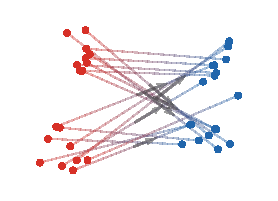
\includegraphics[width=.30\linewidth]{figures/generative-flow-matching-interpolants/product-linear.pdf} &
\index{flow matching}% strictindex
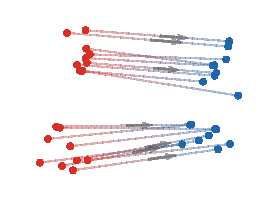
\includegraphics[width=.30\linewidth]{figures/generative-flow-matching-interpolants/ot-linear.pdf} &
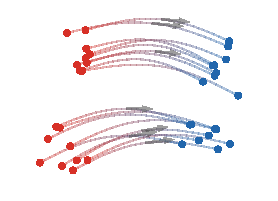
\includegraphics[width=.30\linewidth]{figures/generative-flow-matching-interpolants/curved-bridge.pdf}
\end{tabular}
\caption{\emph{Flow matching interpolants between the same empirical source and target measures.} A product-style random pairing produces crossing paths, an OT pairing gives direct displacement rays, and a curved bridge changes the path geometry while keeping the same endpoints. Gray arrows mark representative midpoint velocities $\partial_t I_t$.}
\label{fig:generative-flow-matching-interpolants}
\end{figure}

\paragraph{Learning a flow field.}
\index{flow matching}% strictindex

This interpolation is not directly useful for sampling from $\beta$, but it can be used to define a flow field $v_t$ so that the Eulerian advection equation~\eqref{eq:eulerian-advection} holds.
%
This flow field is computed by solving an unconstrained least-squares problem, or equivalently, it is a conditional expectation.
\index{conditional!expectation}% strictindex

\begin{prop}[Flow matching vector field]\label{prop-flow-matching-vector-field}
	Assume that $t\mapsto I_t(u)$ is absolutely continuous for $\pi$-almost every $u$, that its derivative $(t,u)\mapsto\partial_t I_t(u)$ is jointly measurable, and that \(\int_0^1\!\int_{\RR^{d'}}\norm{\partial_t I_t(u)}^2\d\pi(u)\d t<+\infty\).
	Let \(U\sim\pi\) and \(X_t=I_t(U)\), so that \(X_t\sim\alpha_t\).
	For almost every $t$, consider the flow-matching problem over \(v_t\in L^2(\alpha_t;\RR^d)\)
\index{flow matching}% strictindex
	\begin{equation}
		\min_{v_t} \int_{\RR^{d'}} \norm{v_t(I_t(u)) - [\partial_t I_t](u)}^2 \, \d\pi(u). \label{eq:flow-matching}
	\end{equation}
	Its minimizer is characterized $\alpha_t$-almost everywhere by
\index{conditional!expectation}% strictindex
	\begin{equation}\label{eq:flow-match-conditional}
		v_t(x)=\EE\bigl[\partial_t I_t(U)\mid X_t=x\bigr].
	\end{equation}
	There is a jointly measurable choice \((t,x)\mapsto v_t(x)\), obtained by disintegrating \(\d t\,\pi(\d u)\) under \((t,u)\mapsto(t,I_t(u))\). For this choice, $v_t\in L^2(\alpha_t;\RR^d)$ for almost every $t$, and the pair $(\alpha_t,v_t)$ satisfies the continuity equation~\eqref{eq:eulerian-advection} in the distributional sense on $(0,1)\times\RR^d$.
\index{continuity equation}% strictindex
\end{prop}

\begin{proof}
	The push-forward identity reads \(\int_{\RR^d}\varphi(x)\,\d\alpha_t(x)=\int_{\RR^{d'}}\varphi(I_t(u))\,\d\pi(u)\) for every bounded continuous test function $\varphi$.
\index{push-forward}% strictindex
	For almost every $t$, the minimizer in~\eqref{eq:flow-matching} is the orthogonal projection in $L^2(\pi;\RR^d)$ of the latent velocity $\partial_t I_t(u)$ onto the closed subspace of functions that depend on $u$ only through $I_t(u)$. This projection is the conditional expectation~\eqref{eq:flow-match-conditional}. Equivalently, disintegration of the joint measure \(\d t\,\pi(\d u)\) by the map \((t,u)\mapsto(t,I_t(u))\) supplies a jointly measurable version. Conditional Jensen gives \(\int\norm{v_t}^2\d\alpha_t\leq\int\norm{\partial_t I_t}^2\d\pi\),
	so the Eulerian velocity is square-integrable in space--time. Its defining conditional-expectation identity is, for every \(m\in L^2(\alpha_t;\RR^d)\),
\index{conditional!expectation}% strictindex
\index{flow matching}% strictindex
	\begin{equation}\label{eq:v_t}
		\int \dotp{m(x)}{v_t(x)} \, \d\alpha_t(x)
		=
		\int \dotp{m(I_t(u))}{[\partial_t I_t](u)} \, \d\pi(u).
	\end{equation}

	We now prove that this field transports the curve $(\alpha_t)_t$. Testing first with \(\varphi\in C_c^\infty(\RR^d)\), and then integrating against compactly supported smooth functions of time, gives the distributional formulation on space--time. The fixed-time weak identity for
	$\partial_t\alpha_t+\diverg(\alpha_t v_t)=0$ is that, for every $\varphi\in C_c^\infty(\RR^d)$,
	\begin{equation}\label{eq:flow-matching-weak-target}
		\frac{\d}{\d t}\int\varphi(x)\,\d\alpha_t(x)
		-
		\int\dotp{v_t(x)}{\nabla\varphi(x)}\,\d\alpha_t(x)
		=0.
	\end{equation}
	By the pathwise chain rule, $t\mapsto\varphi(I_t(u))$ is absolutely continuous for $\pi$-almost every $u$. The space--time integrability assumption and Fubini's theorem justify integration of its derivative, so the push-forward identity gives, for almost every $t$,
\index{push-forward}% strictindex
\index{flow matching}% strictindex
	\begin{equation}\label{eq:flow-matching-test-derivative}
		\frac{\d}{\d t}\int \varphi(x)\d\alpha_t(x)
		=
		\int \dotp{\nabla\varphi(I_t(u))}{[\partial_t I_t](u)}\d\pi(u).
	\end{equation}
	On the other hand, applying~\eqref{eq:v_t} with $m=\nabla\varphi$ gives
	\begin{equation}\label{eq:flow-matching-velocity-test}
		\int\dotp{v_t(x)}{\nabla\varphi(x)}\,\d\alpha_t(x)
		=
		\int \dotp{\nabla\varphi(I_t(u))}{[\partial_t I_t](u)}\d\pi(u).
	\end{equation}
	Comparing~\eqref{eq:flow-matching-test-derivative} and~\eqref{eq:flow-matching-velocity-test} yields~\eqref{eq:flow-matching-weak-target}, which is the desired continuity equation.
\index{continuity equation}% strictindex
\index{flow matching}% strictindex
\end{proof}

\index{conditional!expectation}% strictindex
\index{disintegration}% strictindex
%
Numerically, $(x,t) \mapsto v_t(x)$ can be parameterized by a neural network, for example a U-Net for image data~\citep{RonnebergerFischerBrox2015UNet}. The least-squares regression~\eqref{eq:flow-matching} can then be optimized over the network parameters using stochastic optimization algorithms.
\index{stochastic!gradient}% strictindex
\index{flow matching}% strictindex
%

\paragraph{Sampling algorithm.}
Once the field $v_t$ has been estimated by the tractable regression~\eqref{eq:flow-matching}, generation amounts to integrating its characteristics. For a sufficiently regular version of the exact population field, let $T_t$ denote the flow map solving
\begin{equation}\label{eq-flow-matching-sampling-map}
	\partial_tT_t(x)=v_t(T_t(x)),
	\qquad T_0(x)=x.
\end{equation}
Assume that this ODE generates a unique measurable flow on every compact subinterval of $[0,1)$ and that the continuity equation is unique in the corresponding solution class. Since the exact field transports the prescribed curve, $(T_t)_\sharp\alpha_0=\alpha_t$ for $t<1$. If the flow map extends to $t=1$, then $(T_1)_\sharp\alpha_0=\alpha_1$; consequently, $X_0\sim\alpha_0$ implies $T_1(X_0)\sim\alpha_1$. Numerically, one draws independent samples from the simple reference law $\alpha_0$ and approximates $T_1$ by solving~\eqref{eq-flow-matching-sampling-map} with the regressed field, so the resulting endpoint law is only approximately $\alpha_1$. For singular endpoints, even the exact flow may instead satisfy only $(T_t)_\sharp\alpha_0=\alpha_t\rightharpoonup\alpha_1$ as $t\uparrow1$, while the velocity or its spatial derivative becomes singular.
\index{transport!map}% strictindex
\index{continuity equation}% strictindex

This inference stage can be expensive because every generated sample requires many neural-field evaluations along an ODE trajectory. Section~\ref{sec-one-step-generative-models} presents the opposite tradeoff: repeated flow estimation or distillation makes training more expensive, but the final sampler is a single network evaluation.

\paragraph{Connection with diffusion models.}\label{par-diffusion-model-connection}
\index{diffusion model}% strictindex

Diffusion models generate data by reversing a progressive noising process. Complementary applied and SDE-based introductions are given by \citet{HighamHighamGrindrod2025DiffusionIntroduction} and \citet{TangZhao2025DiffusionTutorial}. Here we focus on their connection with the interpolants and velocity regression introduced above.

In the special case where $I_t(x,y)=(1-t)x+ty$ is a linear interpolation and $\pi = \alpha_0 \otimes \alpha_1$, the curve $\alpha_t$ is a convolution of rescaled versions of $\alpha_0$ and $\alpha_1$, since convolution is the law of a sum of independent random vectors. The flow-matching problem~\eqref{eq:flow-matching} becomes
\index{flow matching}% strictindex
\[
    \min_{(v_t)_t} \int_0^1\!\int_{\RR^{d} \times \RR^d} \norm{v_t( (1-t)x+t y ) - (y-x) }^2 \, \d\alpha_0(x) \d\alpha_1(y)\,\d t.
\]
When one endpoint is an isotropic Gaussian, this construction is closely related to the probability-flow formulation of diffusion models, up to the usual change of time parametrization~\citep{Song2021ScoreSDE}. This is why flow matching can be viewed both as a deterministic alternative to diffusion training and as a common language for diffusion paths, OT-inspired paths, and rectified paths~\citep{Lipman2022FlowMatching,Liu2023RectifiedFlow,Albergo2025StochasticInterpolants}. The next two propositions are written in the noising direction, from a data law $\alpha$ to a Gaussian; reversing time gives the corresponding sampling flow. They also give an explicit closed form for $v_t$ and show that it is a gradient field.
\index{flow!probability ODE}% strictindex
\index{diffusion model}% strictindex

Figure~\ref{fig:generative-diffusion-2d-forward-backward} illustrates at this point how the scalar coefficients of the interpolant separately control contraction of the data centers and growth of the Gaussian noise.

\begin{figure}[ht]
\centering
\begin{tabular}{@{}c@{}}
\small linear bridge, $a_t=1-t$, $b_t=t$ \\[-.15em]
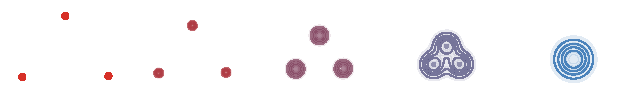
\includegraphics[width=.72\linewidth]{figures/generative-diffusion-2d-forward-backward/forward-density-linear.pdf} \\[.15em]
\small OU/variance-preserving bridge, $a_t=\cos(\pi t/2)$, $b_t=\sin(\pi t/2)$ \\[-.15em]
\index{bridge!OU}% strictindex
\index{bridge!variance-preserving}% strictindex
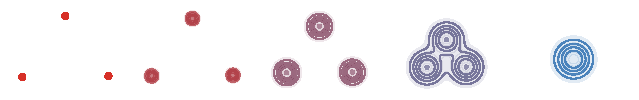
\includegraphics[width=.72\linewidth]{figures/generative-diffusion-2d-forward-backward/forward-density-ou.pdf}
\end{tabular}
\caption{\emph{Two-dimensional noising paths from three Dirac masses to a single Gaussian.} The top row shows the linear interpolation $X_t=(1-t)X_0+tZ$, whose component centers move linearly toward the origin and whose covariance grows like $(t\sigma)^2\Id$. The bottom row uses the variance-preserving Ornstein--Uhlenbeck coefficients $a_\tau=e^{-\tau}$ and $b_\tau=\sqrt{1-e^{-2\tau}}$, reparametrized by $\tau=-\log\cos(\pi t/2)$ so that $a_t=\cos(\pi t/2)$ and $b_t=\sin(\pi t/2)$. It has the same endpoints but a different speed of contraction and noising.}
\index{Ornstein-Uhlenbeck@Ornstein--Uhlenbeck!process}% strictindex
\label{fig:generative-diffusion-2d-forward-backward}
\end{figure}
%
For the isotropic Gaussian endpoint considered next, $v_t$ belongs to the tangent-gradient space~\eqref{eq-wasserstein-tangent-space} and is also the minimum-energy velocity of~\eqref{eq:least-square-field}. The regression~\eqref{eq:flow-matching} is computationally simpler because the continuity equation has already been enforced by the chosen interpolant.
\index{continuity equation}% strictindex
%
To prove this, we rely on Tweedie's formula~\citep{Efron2011Tweedie}, which expresses the optimal Gaussian denoiser through the score, i.e.\ the gradient of the log-density.
\index{Gaussian!denoiser}% strictindex
\index{score function}% strictindex
\index{Tweedie identity}% strictindex

\begin{proposition}[Tweedie identity]\label{prop:Tweedie}
Let $W$ be a random vector in $\RR^{d}$ with law $\beta\in\Pp_1(\RR^d)$.
For $\sigma>0$, let $Z\sim\Gaussian(0,\Id)$ be independent of $W$ and observe
\[
Y=W+\sigma Z.
\]
Denote by $\rho_\sigma$ the smooth positive density of \(\beta_\sigma=\beta * \Gaussian(0,\sigma^{2}\Id)\), which is the law of $Y$.
Then the conditional mean admits the following everywhere-defined version:
\[
\EE\bigl[W\mid Y=y\bigr]
      =y+\sigma^{2}\nabla \log \rho_\sigma(y)
\qquad\text{for all } y \in \RR^{d}.
\]
\end{proposition}

\begin{proof}
Let $\varphi_\sigma$ be the $\Gaussian(0,\sigma^{2}\Id)$ density. Bayes' rule gives \(\EE[W\mid Y=y]=\rho_\sigma(y)^{-1}\int_{\RR^{d}} w\varphi_\sigma(y-w)\,\d\beta(w)\).
Differentiating the Gaussian convolution under the integral sign and using
$
\nabla_y\varphi_\sigma(y-w)
     = -\sigma^{-2}(y-w)\,\varphi_\sigma(y-w)
$
yields
\[
\nabla\rho_\sigma(y)
= \int \nabla_y\varphi_\sigma(y-w)\,\d\beta(w)
= -\sigma^{-2}\Bigl(y-\EE[W\mid Y=y]\Bigr)\,\rho_\sigma(y).
\]
Rearranging finishes the proof.
\end{proof}


Tweedie's identity now turns the conditional expectation defining flow matching into an explicit score field for a Gaussian endpoint.

\begin{proposition}[Gaussian-endpoint flow-matching field]\label{prop:flow}
\index{flow matching}% strictindex
Let \(\alpha\in\Pp_2(\RR^d)\), let $X_0\sim\alpha$, and let $Z\sim\Gaussian(0,\Id)$ be independent.
For $t\in(0,1)$ set \(X_t=(1-t)X_0+tZ\) and \(\alpha_t=\operatorname{Law}(X_t)=\rho_t\,\d x\). The minimizer $v^\star:\RR^d\times(0,1)\to\RR^d$ of the flow-matching regression~\eqref{eq:flow-matching} is
\[
v^\star(x,t)
= -\frac{1}{1-t}\,x \;-\; \frac{t}{1-t}\,\nabla\log\rho_t(x)
\qquad (x\in\RR^{d},\;t\in(0,1)).
\]
In particular, for each $t\in(0,1)$ this field is the gradient field \(v^\star(\cdot,t)=-\nabla\bigl(\norm{\cdot}^2/[2(1-t)]+t\log\rho_t/(1-t)\bigr)\).
\end{proposition}

\begin{proof}
Fix $t\in(0,1)$ and write $W=(1-t)X_0$ and $\sigma=t$, so that
$X_t=W+\sigma Z$ matches the setting of Proposition~\ref{prop:Tweedie}.
\index{Tweedie identity}% strictindex
Conditional expectations satisfy
\index{conditional!expectation}% strictindex
$
v^\star(x,t)
= \EE[Z-X_0\mid X_t=x]
= \frac{1}{t}\,\EE[X_t-W\mid X_t=x]
  -\,\frac{1}{1-t}\,\EE[W\mid X_t=x].
$
Applying Proposition~\ref{prop:Tweedie} to $\EE[W\mid X_t=x]$ and
\index{Tweedie identity}% strictindex
noting $\EE[Z\mid X_t=x]=-t\nabla\log\rho_t(x)$
gives the claimed formula.
\end{proof}

Figure~\ref{fig:generative-diffusion-1d-forward-backward} shows both directions of this construction: the prescribed interpolation noising the data and the same probability-flow ODE integrated backward for sampling.

\begin{figure}[ht]
\centering
\begin{tabular}{@{}cc@{}}
\small forward noising & \small reverse probability flow \\[-.15em]
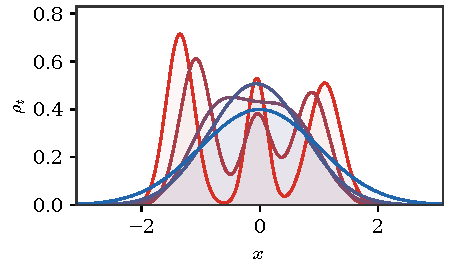
\includegraphics[width=.37\linewidth]{figures/generative-diffusion-1d-forward-backward/forward-densities.pdf} &
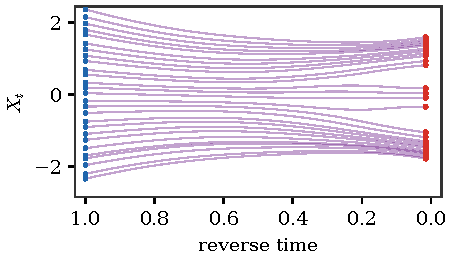
\includegraphics[width=.37\linewidth]{figures/generative-diffusion-1d-forward-backward/backward-trajectories.pdf}
\end{tabular}
\caption{\emph{One-dimensional diffusion bridge for a Gaussian-mixture data law.} The forward path $X_t=(1-t)X_0+tZ$ smooths the red data density toward a blue Gaussian endpoint. Reversing the probability-flow ODE transports stratified, slightly jittered seeds representing that endpoint back toward the data modes, making the splitting of trajectories across mixture components visible.}
\index{Gaussian!mixture}% strictindex
\index{flow!probability ODE}% strictindex
\label{fig:generative-diffusion-1d-forward-backward}
\end{figure}

The same probability-flow intuition is explicit in two dimensions. For a discrete data law, or more generally for a Gaussian mixture, the noising density is a Gaussian mixture whose score can be evaluated in closed form. More precisely, if $\alpha_0=\sum_j w_j\Gaussian(c_j,\Sigma_j)$ and $Z\sim\Gaussian(0,\sigma^2\Id)$ is independent of $X_0$, then $X_t=a_tX_0+b_tZ$ has component means $a_t c_j$ and covariances $a_t^2\Sigma_j+b_t^2\sigma^2\Id$. Dirac data correspond to $\Sigma_j=0$; only in that case does the linear bridge reduce to $\alpha_t=\sum_jw_j\Gaussian((1-t)c_j,(t\sigma)^2\Id)$. If $\rho_t$ denotes its density and $s_t=\nabla\log\rho_t$ its score, the scaled version of Proposition~\ref{prop:flow} gives $v_t(x)=-(x+t\sigma^2s_t(x))/(1-t)$.
\index{noising schedule}% strictindex
\index{score function}% strictindex

\paragraph{When is the induced map optimal?}

Integrating the learned velocity gives a deterministic map from $\alpha_0$ to $\alpha_1$, but this map is not automatically the Brenier optimal map. It is optimal only in special cases where the accumulated flow remains the gradient of a convex potential. The Gaussian product-coupling case already shows the precise obstruction: the interpolated covariances are simple, the velocity is affine, but the terminal map can contain a hidden rotational part. This phenomenon, and its extensions to rectified flows and mixtures, is analyzed in depth in~\citet{HertrichChambolleDelon2025RectifiedOT}.
\index{convex!potential}% strictindex
\index{product!coupling}% strictindex
\index{flow!rectified}% strictindex
Quadratic optimal transport between Gaussian measures is developed in Section~\ref{sec-gaussian-bures}; in particular, Proposition~\ref{prop-gaussian-w2-bures} and~\eqref{eq-bures-map} prove the formula for $T^{\rm OT}$ used below.

\begin{prop}[Gaussian flow matching and optimality]\label{prop-gaussian-flow-matching-optimality}
\index{Gaussian!flow matching}% strictindex
	Let $\Sigma_0,\Sigma_1\succ0$ and let $X_0\sim\Gaussian(0,\Sigma_0)$ and $X_1\sim\Gaussian(0,\Sigma_1)$ be independent. Consider the linear flow-matching interpolation
\index{flow matching}% strictindex
	\[
		X_t=(1-t)X_0+tX_1,
		\qquad
		\alpha_t=\operatorname{Law}(X_t)=\Gaussian(0,\Sigma_t),
	\]
	where $\Sigma_t=(1-t)^2\Sigma_0+t^2\Sigma_1$. Then the exact flow-matching velocity is affine, $v_t(x)=A_tx$, with $A_t=\bigl(t\Sigma_1-(1-t)\Sigma_0\bigr)\Sigma_t^{-1}$.
\index{flow matching}% strictindex
	The induced flow map $T_t^{\rm FM}$ from $\alpha_0$ to $\alpha_t$ is
\index{flow!map}% strictindex
	\begin{equation}\label{eq-gaussian-product-fm-map}
		T_t^{\rm FM}
		=
		\Sigma_0^{1/2}
		\Bigl((1-t)^2\Id+t^2\Sigma_0^{-1/2}\Sigma_1\Sigma_0^{-1/2}\Bigr)^{1/2}
		\Sigma_0^{-1/2}.
	\end{equation}
	\eqllead{In particular,}{eq-gaussian-product-fm-terminal-map}{
		T_1^{\rm FM}
		=
		\Sigma_0^{1/2}
		\bigl(\Sigma_0^{-1/2}\Sigma_1\Sigma_0^{-1/2}\bigr)^{1/2}
		\Sigma_0^{-1/2}.
	}
	This terminal map coincides with the quadratic optimal transport map
\index{transport!map}% strictindex
	\begin{equation}\label{eq-gaussian-brenier-map-comparison}
		T^{\rm OT}
		=
		\Sigma_0^{-1/2}
		\bigl(\Sigma_0^{1/2}\Sigma_1\Sigma_0^{1/2}\bigr)^{1/2}
		\Sigma_0^{-1/2}
	\end{equation}
	if and only if $\Sigma_0\Sigma_1=\Sigma_1\Sigma_0$.
\end{prop}

\begin{proof}
	The conditional-expectation formula gives
\index{conditional!expectation}% strictindex
	\(v_t(x)=\EE[X_1-X_0\mid X_t=x]\).
	Since all variables are jointly Gaussian, this conditional expectation is linear and
	\[
		v_t(x)
		=
		\operatorname{Cov}(X_1-X_0,X_t)\operatorname{Cov}(X_t)^{-1}x
		=
		\bigl(t\Sigma_1-(1-t)\Sigma_0\bigr)\Sigma_t^{-1}x,
	\]
		which proves the stated velocity formula. To solve the characteristic equation, whiten the source by setting \(C=\Sigma_0^{-1/2}\Sigma_1\Sigma_0^{-1/2}\) and \(\widetilde X_t=\Sigma_0^{-1/2}X_t\).
	In these coordinates the source covariance is $\Id$ and
	\(\widetilde\Sigma_t=(1-t)^2\Id+t^2C\).
	Because $\Id$ and $C$ commute, the affine flow map in whitened coordinates is simply $\widetilde T_t=\widetilde\Sigma_t^{1/2}$. Indeed,
\index{flow!map}% strictindex
	$\frac{\d}{\d t}\widetilde\Sigma_t^{1/2}=\bigl(tC-(1-t)\Id\bigr)\widetilde\Sigma_t^{-1/2}$, which is exactly the equation $\dot{\widetilde T}_t=\widetilde A_t\widetilde T_t$ with $\widetilde T_0=\Id$. Returning to the original coordinates gives~\eqref{eq-gaussian-product-fm-map}, and $t=1$ gives~\eqref{eq-gaussian-product-fm-terminal-map}.

		Both $T_1^{\rm FM}$ and $T^{\rm OT}$ push $\Gaussian(0,\Sigma_0)$ to $\Gaussian(0,\Sigma_1)$. The Brenier map between nondegenerate Gaussians is the unique symmetric positive definite linear map with this property. Hence $T_1^{\rm FM}=T^{\rm OT}$ if and only if $T_1^{\rm FM}$ is symmetric positive definite. The map $T_1^{\rm FM}$ is similar to $C^{1/2}$, so if it is symmetric then it is automatically positive definite. It remains to characterize symmetry. Since $C^{1/2}$ is symmetric positive definite, \((T_1^{\rm FM})^\top=\Sigma_0^{-1/2}C^{1/2}\Sigma_0^{1/2}\).
\index{Brenier!map}% strictindex
	Thus symmetry of $T_1^{\rm FM}$ is equivalent to
	$\Sigma_0 C^{1/2}=C^{1/2}\Sigma_0$, hence to $\Sigma_0 C=C\Sigma_0$ by functional calculus. Multiplying this identity on the left and right by $\Sigma_0^{1/2}$ gives $\Sigma_0\Sigma_1=\Sigma_1\Sigma_0$. Conversely, if $\Sigma_0$ and $\Sigma_1$ commute, they are orthogonally co-diagonalizable, and both~\eqref{eq-gaussian-product-fm-terminal-map} and~\eqref{eq-gaussian-brenier-map-comparison} reduce in that basis to the diagonal map with entries $\sqrt{\lambda_{1,k}/\lambda_{0,k}}$. This proves the equivalence.
\end{proof}

The proposition gives a compact warning about a common overinterpretation of flow matching.

\begin{rem}[Changing the bridge speed does not restore optimality]
	The same terminal map~\eqref{eq-gaussian-product-fm-terminal-map} is obtained for every continuously differentiable scalar schedule $X_t=a_tX_0+b_tX_1$ satisfying $(a_0,b_0)=(1,0)$, $(a_1,b_1)=(0,1)$, and $a_t^2\Id+b_t^2C\succ0$ for all $t$. Indeed, after whitening, the covariance path is $a_t^2\Id+b_t^2C$, and the flow map is its positive square root. Thus changing the speed of a nondegenerate scalar Gaussian bridge, for instance by using an OU schedule, cannot repair the non-optimality created by non-commuting covariances.
	Commuting covariances reduce the terminal map to independent one-dimensional scalings, whereas non-commuting covariances create a non-symmetric affine map, hence a transport with a rotational or shearing component. More generally, mixture-like paths can create the same obstruction even when every instantaneous velocity looks natural. This distinction is closely related to counterexamples showing that flow maps associated with Fokker--Planck or diffusion-type evolutions do not in general provide optimal transport maps~\citep{LavenantSantambrogio2022FlowMap}. In particular, starting from an isotropic Gaussian does not by itself guarantee optimality once the target distribution is non-Gaussian; additional structural assumptions on the path or on the coupling are needed.
\end{rem}
\index{affine!map}% strictindex
\index{flow!map}% strictindex
\index{rotational component}% strictindex
\index{shearing component}% strictindex
\index{transport!map}% strictindex
\index{Fokker-Planck@Fokker--Planck!equation}% strictindex
\index{flow matching}% strictindex
\index{Gaussian!flow matching}% strictindex
\index{covariance!commuting}% strictindex

\paragraph{Variations on the interpolant.}
\index{noising path}% strictindex
\index{bridge!OU}% strictindex
\index{bridge!overshooting}% strictindex
\index{interpolant}% strictindex
\index{bridge!speed}% strictindex

The geometry of the generated trajectories depends on the chosen interpolant, not only on the two endpoint laws. There is first a harmless ambiguity: a monotone reparametrization $X_t=(1-\lambda(t))X_0+\lambda(t)X_1$ of the linear bridge only changes the speed of the flow,
\index{bridge!linear}% strictindex
\index{time reparametrization}% strictindex
\[
	v_t(x)=\lambda'(t)\,v^{\rm lin}_{\lambda(t)}(x),
	\qquad
	v^{\rm lin}_{r}(x)=\EE[X_1-X_0\mid (1-r)X_0+rX_1=x].
\]
It therefore leaves the spatial integral curves unchanged. A diffusion model instead prescribes a forward stochastic noising process, learns its score or reverse drift, and samples by integrating the reverse SDE or the associated probability-flow ODE~\citep{Song2021ScoreSDE}. Although its path law is genuinely stochastic, its one-time marginals can coincide with those of a static Gaussian interpolant.
\index{diffusion model}% strictindex
\index{noising path}% strictindex

\begin{prop}[Static Gaussian interpolants and Ornstein--Uhlenbeck noising]\label{prop-static-ou-equivalence}
	Let $\alpha\in\Pp_2(\RR^d)$ and $\sigma>0$. Let $X_0\sim\alpha$ and $Z\sim\Gaussian(0,\sigma^2\Id)$ be independent, and set $X_t=a_tX_0+b_tZ$ on an open time interval where the differentiable scalar functions satisfy $a_t>0$ and $b_t>0$. If $\rho_t$ is the density of $X_t$, then its flow-matching velocity is
	\begin{equation}\label{eq-scalar-gaussian-interpolant-velocity}
		v_t(x)=\frac{\dot a_t}{a_t}x+
		\left(\frac{\dot a_t b_t^2}{a_t}-\dot b_t b_t\right)\sigma^2\nabla\log \rho_t(x).
	\end{equation}
	For the variance-preserving coefficients $a_\tau=e^{-\tau}$ and $b_\tau=\sqrt{1-e^{-2\tau}}$, with $\tau>0$, these marginals are exactly those of the Ornstein--Uhlenbeck diffusion
	\begin{equation}\label{eq-ou-forward-diffusion}
		\d X_\tau^{\rm OU}=-X_\tau^{\rm OU}\d\tau+\sqrt{2}\,\sigma\d B_\tau,
		\qquad X_0^{\rm OU}\sim\alpha,
	\end{equation}
	and~\eqref{eq-scalar-gaussian-interpolant-velocity} reduces to $v_\tau(x)=-x-\sigma^2\nabla\log \rho_\tau(x)$. Moreover, the finite-time coefficients $a_t=\cos(\pi t/2)$ and $b_t=\sin(\pi t/2)$ describe the same marginal curve after the time change $\tau=-\log\cos(\pi t/2)$.
\end{prop}

\begin{proof}
	Tweedie's identity gives
	\[
	\EE[X_0\mid X_t=x]=a_t^{-1}(x+b_t^2\sigma^2\nabla\log\rho_t(x)),
	\qquad
	\EE[Z\mid X_t=x]=-b_t\sigma^2\nabla\log\rho_t(x).
	\]
	Substitution in $v_t(x)=\dot a_t\EE[X_0\mid X_t=x]+\dot b_t\EE[Z\mid X_t=x]$ proves~\eqref{eq-scalar-gaussian-interpolant-velocity}. The explicit solution of~\eqref{eq-ou-forward-diffusion} is $X_\tau^{\rm OU}=e^{-\tau}X_0^{\rm OU}+\sqrt{2}\,\sigma\int_0^\tau e^{-(\tau-s)}\d B_s$. The noise term $\sqrt{2}\,\sigma\int_0^\tau e^{-(\tau-s)}\d B_s$ is independent of $X_0^{\rm OU}$ and Gaussian with covariance $\sigma^2(1-e^{-2\tau})\Id$, proving equality of the one-time marginals. Substituting the OU coefficients in~\eqref{eq-scalar-gaussian-interpolant-velocity} gives the stated velocity, and the trigonometric parametrization follows from $e^{-\tau}=\cos(\pi t/2)$.
\end{proof}
\index{Tweedie identity}% strictindex
\index{Ornstein-Uhlenbeck@Ornstein--Uhlenbeck!process}% strictindex
\index{bridge!variance-preserving}% strictindex
\index{Fokker-Planck@Fokker--Planck!equation}% strictindex

For the linear bridge, $a_t=1-t$ and $b_t=t$, Proposition~\ref{prop-static-ou-equivalence} recovers Proposition~\ref{prop:flow}. For Ornstein--Uhlenbeck (OU) noising, sampling integrates the probability-flow ODE backward in $\tau$; the same law evolves forward according to the OU Fokker--Planck equation. Numerically, integration is stopped at a small positive noising time before a singular data endpoint. A genuinely different scalar bridge uses $a_t=(1-t)(1-2t)$ and $b_t=t$. Its data coefficient changes sign before vanishing, so the intermediate mixture reflects through the origin and produces visibly different reverse trajectories.
\index{scalar bridge}% strictindex
\index{time change}% strictindex
\index{bridge!overshooting}% strictindex

Figure~\ref{fig:generative-diffusion-schedule-comparison} places the quadratic-OT rays and three reverse-flow schedules side by side.

\begin{figure}[htbp]
\centering
{\setlength{\tabcolsep}{.12em}
\begin{tabular}{@{}cccc@{}}
\small OT rays & \small linear bridge & \small OU VP bridge & \small overshooting bridge \\[-.15em]
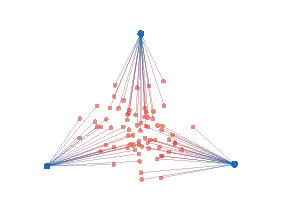
\includegraphics[width=.23\linewidth]{figures/generative-diffusion-versus-ot-2d/ot-rays.pdf} &
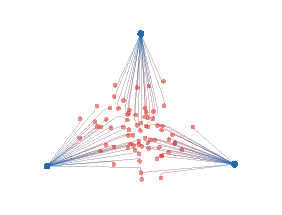
\includegraphics[width=.23\linewidth]{figures/generative-diffusion-versus-ot-2d/schedule-linear.pdf} &
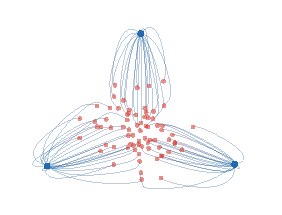
\includegraphics[width=.23\linewidth]{figures/generative-diffusion-versus-ot-2d/schedule-vp.pdf} &
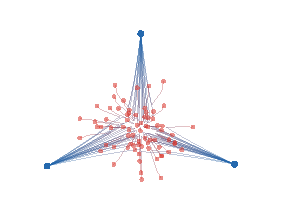
\includegraphics[width=.23\linewidth]{figures/generative-diffusion-versus-ot-2d/schedule-overshoot.pdf}
\end{tabular}}
\caption{\emph{Quadratic-OT rays and exact reverse-flow trajectories for three interpolants.} All four panels use the same three-Dirac target and centered Gaussian source. From left to right: straight displacement rays selected by quadratic OT; the linear bridge $a_t=1-t$, $b_t=t$; the variance-preserving OU bridge $a_\tau=e^{-\tau}$, $b_\tau=\sqrt{1-e^{-2\tau}}$; and the overshooting bridge $a_t=(1-t)(1-2t)$, $b_t=t$. The last bridge is not a time reparametrization of the preceding two and bends the trajectories more strongly.}
\index{Gaussian!mixture}% strictindex
\index{bridge!OU}% strictindex
\index{bridge!variance-preserving}% strictindex
\index{flow!probability ODE}% strictindex
\index{score function}% strictindex
\index{flow!reverse}% strictindex
\label{fig:generative-diffusion-schedule-comparison}
\end{figure}

\paragraph{Stochastic interpolants.}
\index{stochastic!interpolant}% strictindex
\index{latent!variable}% strictindex
\index{flow!probability ODE}% strictindex
The deterministic construction of Definition~\ref{def-deterministic-interpolant} can be enriched by a static Gaussian perturbation whose amplitude varies along the interpolation. In the construction of Albergo, Boffi and Vanden-Eijnden~\citep{Albergo2025StochasticInterpolants}, one auxiliary Gaussian variable is shared by the entire path.
\begin{defn}[Stochastic interpolant]\label{def-stochastic-interpolant}
Let $(X_0,X_1)\sim\pi\in\Couplings(\alpha_0,\alpha_1)$, let $Z\sim\Gaussian(0,\Id)$ be independent of $(X_0,X_1)$, and let $I_t$ be a deterministic interpolant for this coupling. Given an absolutely continuous noise schedule $\gamma:[0,1]\to\RR$ satisfying $\gamma(0)=\gamma(1)=0$, the stochastic interpolant is
\begin{equation}\label{eq-static-noise-stochastic-interpolant}
	X_t=I_t(X_0,X_1)+\gamma(t)Z,
	\qquad \alpha_t=\operatorname{Law}(X_t).
\end{equation}
Assume in addition that $\EE\int_a^b\norm{\partial_tI_t(X_0,X_1)+\dot\gamma(t)Z}^2\,\d t<+\infty$ for every $0<a<b<1$.
\end{defn}
The same draw of $Z$ is used for every $t$: conditionally on $(X_0,X_1,Z)$, the path remains absolutely continuous. Thus~\eqref{eq-static-noise-stochastic-interpolant} is the push-forward construction~\eqref{eq:interp-coupling} with latent variable $u=(X_0,X_1,Z)$. Its Eulerian velocity is
\[
	v_t(x)=\EE\bigl[\partial_tI_t(X_0,X_1)+\dot\gamma(t)Z\mid X_t=x\bigr],
\]
and Proposition~\ref{prop-flow-matching-vector-field}, applied on compact subintervals of $(0,1)$, gives the associated continuity equation. Local rather than endpoint-uniform square integrability includes the common schedule $\gamma(t)=\sqrt{t(1-t)}$, whose derivative is integrable but not square-integrable near the endpoints. The endpoint laws still follow by continuity of the interpolant. When regularity permits their construction, the associated SDEs are alternative dynamics with the same one-time marginals; they are not obtained by replacing $Z$ with independent noise at every time.

\begin{rem}[Brownian realizations of interpolant marginals]\label{rem-noisy-stochastic-interpolants}
\index{stochastic!interpolant}% strictindex
\index{Fokker-Planck@Fokker--Planck!equation}% strictindex
\index{flow!probability ODE}% strictindex
One can instead realize an interpolating marginal curve by Brownian-in-time dynamics. This gives a different path law from Definition~\ref{def-stochastic-interpolant}, although the one-time marginals can coincide, as in Proposition~\ref{prop-static-ou-equivalence}. The static-noise paths are absolutely continuous, whereas nondegenerate diffusion paths have nonzero quadratic variation. Let
\[
	\d X_t=r_t(U,X_t)\d t+\sigma_t(U,X_t)\d B_t,
	\qquad \alpha_t=\operatorname{Law}(X_t),
\]
where $U\sim\pi$ is static and independent of the Brownian motion $B_t$. Assume the SDE is well posed, adapted, and has locally integrable drift and quadratic variation so that the following It\^o calculation is justified. Conditioning on the observed state defines
\[
	v_t(x)=\EE\bigl[r_t(U,X_t)\mid X_t=x\bigr],
	\qquad
	D_t(x)=\EE\bigl[\sigma_t(U,X_t)\sigma_t(U,X_t)^\top\mid X_t=x\bigr].
\]
For smooth test functions $\varphi$,
\[
	\frac{\d}{\d t}\int\varphi\d\alpha_t
	=
	\int\dotp{\nabla\varphi}{v_t}\d\alpha_t
	+
	\frac12\int\tr(D_t\nabla^2\varphi)\d\alpha_t,
\]
or, in distributional form,
\begin{equation}\label{eq:noisy-interpolant-fokker-planck}
	\partial_t\alpha_t+\diverg(\alpha_tv_t)
	=
	\frac12\sum_{i,j}\partial_{i,j}^2\bigl((D_t)_{i,j}\alpha_t\bigr).
\end{equation}
The noisy analogue of~\eqref{eq:flow-matching} therefore regresses the drift through $\min_w\EE[\norm{w_t(X_t)-r_t(U,X_t)}^2]$. It learns a Fokker--Planck drift rather than a pure continuity-equation velocity. If $\alpha_t=\rho_t\d x$ has a smooth positive density, the same marginal curve has the formal probability-flow representation $\partial_t\rho_t+\diverg(\rho_t\bar v_t)=0$, where $\bar v_t=v_t-(2\rho_t)^{-1}\diverg(\rho_tD_t)$ and the matrix divergence is taken row-wise. For a spatially constant diffusion matrix $D_t(x)=\sigma_t^2\Id$, this becomes $\bar v_t=v_t-(\sigma_t^2/2)\nabla\log\rho_t$.
\index{flow!probability ODE}% strictindex
\end{rem}

% -----------------------------------------------------------------------------

\subsection{One-Step Generative Models}
\label{sec-one-step-generative-models}
\index{one-step generative model}% strictindex

One-step generative models try to keep the geometric training principle of flows while removing expensive multi-step integration at sampling time. To expose this tradeoff, we first describe direct non-parametric sampling by a Wasserstein flow; the subsequent constructions move that evolution into training and store its endpoint in a single generator evaluation.
\index{generative model}% strictindex

\paragraph{Non-parametric sampling via gradient flow.}
\index{Wasserstein!gradient flow}% strictindex
\index{particle!gradient flow}% strictindex
Let $\beta$ be the target law and let $\mathcal D\geq0$ be a discrepancy with $\mathcal D(\alpha,\beta)=0$ if and only if $\alpha=\beta$. Define
\begin{equation}\label{eq-one-step-discrepancy-energy}
	f_\beta(\alpha)\eqdef\mathcal D(\alpha,\beta).
\end{equation}
A direct sampling strategy follows the formal $\Wass_2$ gradient flow
\begin{equation}\label{eq-nonparametric-discrepancy-flow}
	\partial_t\alpha_t+\diverg(\alpha_t v_t)=0,
	\qquad
	v_t=-\Wgrad f_\beta(\alpha_t)
	=-\nabla\delta f_\beta(\alpha_t).
\end{equation}
If this flow is globally well posed and converges to a global minimizer of $f_\beta$, then its limit is $\beta$. These are substantial assumptions, not automatic consequences of the definition of a discrepancy. If $\alpha_0=n^{-1}\sum_{i=1}^n\delta_{X_i(0)}$ and the dynamics preserves empirical measures, then~\eqref{eq-nonparametric-discrepancy-flow} becomes the particle system
\begin{equation}\label{eq-nonparametric-particle-flow}
	\dot X_i(t)=v_t(X_i(t))
	=-\Wgrad f_\beta(\alpha_t)(X_i(t)),
	\qquad
	\alpha_t=\frac1n\sum_{i=1}^n\delta_{X_i(t)}.
\end{equation}
For fixed $n$, such a curve cannot converge weakly to a non-atomic target while retaining exactly $n$ equally weighted atoms. The sampling interpretation is therefore a large-particle approximation: one evolves a sufficiently rich cloud and lets $n$ increase. This approach is most practical in low dimension because it stores and repeatedly updates many interacting particles, in sharp contrast with flow matching, which learns a field that can subsequently transport arbitrary fresh samples.

For example, the squared Wasserstein loss moves a diffuse source toward the target along a time-reparametrized displacement interpolation. With an MMD loss, the interaction field derived in Section~\ref{sec-wasserstein-gradient-flows} instead moves particles according to kernel discrepancies. These choices give different trajectories even when the target law is the same; convergence must be studied for the chosen energy.

\paragraph{One-step models via parameter-domain discrepancy flows.}
\index{one-step generative model}% strictindex
\index{flow!parameter-domain}% strictindex
\index{discrepancy minimization}% strictindex
\index{minibatch bias}% strictindex
\index{parameter space}% strictindex
\index{minibatch}% strictindex
\index{Wasserstein!GAN}% strictindex
\index{MMD-GAN}% strictindex

The most direct one-step strategy is to train the generator parameters themselves by descending the discrepancy~\eqref{eq-one-step-discrepancy-energy}. Let $\zeta$ be a simple latent distribution and let $G_\theta:\Zz\to\RR^d$ be a neural generator on a standard Borel latent space $\Zz$. The objective is to find $\theta$ such that $(G_\theta)_\sharp\zeta=\beta$, or, in practice, such that the generated law is close to $\beta$. Define
\begin{equation}\label{eq-one-step-parameter-discrepancy}
	H_\beta(\theta)
	\eqdef
	f_\beta\big((G_\theta)_\sharp\zeta\big)
	=
	\mathcal D\big((G_\theta)_\sharp\zeta,\beta\big).
\end{equation}
This viewpoint includes Wasserstein GANs, MMD-GANs and Sinkhorn generative models~\citep{WassersteinGAN,MMD-GAN,2017-Genevay-AutoDiff}; when $\mathcal D$ is written through a dual potential or discriminator, it gives an adversarial formulation in which a discriminator represents that dual potential. The resulting training dynamics is the ordinary Euclidean gradient flow in parameter space,
\begin{equation}\label{eq-one-step-parameter-flow}
	\dot\theta_t=-\nabla_\theta H_\beta(\theta_t).
\end{equation}
This parameter flow induces a flow of generated measures, but this induced flow is not intrinsic in general. Set
\[
	\alpha_t\eqdef(G_{\theta_t})_\sharp\zeta,
	\qquad
	X_t=G_{\theta_t}(Z),
	\qquad
	Z\sim\zeta.
\]
\begin{prop}[Velocity induced by a parameter path]\label{prop-parameter-path-continuity}
	Assume that $t\mapsto\theta_t$ is continuously differentiable on $[0,T]$, and that, for $\zeta$-almost every $z$, the map $\theta\mapsto G_\theta(z)$ is continuously differentiable. Assume also that $(t,z)\mapsto\partial_\theta G_{\theta_t}(z)$ is jointly measurable and that
	\[
		\int_0^T\!\int_\Zz
		\norm{\partial_\theta G_{\theta_t}(z)\dot\theta_t}
		\,\d\zeta(z)\d t<+\infty.
	\]
	Let $\eta_{t,x}$ be a jointly measurable disintegration of $\d t\,\zeta(\d z)$ under $(t,z)\mapsto(t,G_{\theta_t}(z))$. Then the Eulerian velocity
	\begin{equation}\label{eq-one-step-induced-velocity}
		v_t(x)=\int \partial_\theta G_{\theta_t}(z)\dot\theta_t\,\d\eta_{t,x}(z)
	\end{equation}
		satisfies, in the distributional sense on $(0,T)\times\RR^d$,
	\begin{equation}\label{eq-one-step-induced-continuity}
		\partial_t\alpha_t+\diverg(\alpha_t v_t)=0.
	\end{equation}
	If $\theta_t$ follows~\eqref{eq-one-step-parameter-flow}, then $\dot\theta_t=-\nabla_\theta H_\beta(\theta_t)$ in~\eqref{eq-one-step-induced-velocity}.
\end{prop}

\begin{proof}
	The chain rule gives $\dot X_t=\partial_\theta G_{\theta_t}(Z)\dot\theta_t$. For every bounded measurable $\psi$, disintegration means
	\[
		\int \psi(z)\,\d\zeta(z)=\int_{\RR^d}\left(\int \psi(z)\,\d\eta_{t,x}(z)\right)\d\alpha_t(x)
	\]
	for almost every $t$. Consequently, for every smooth compactly supported $\varphi$,
	\[
		\frac{\d}{\d t}\int \varphi(x)\,\d\alpha_t(x)
		=
		\int \dotp{\nabla\varphi(x)}{v_t(x)}\,\d\alpha_t(x),
	\]
	which is the weak form of~\eqref{eq-one-step-induced-continuity}.
\end{proof}

The velocity~\eqref{eq-one-step-induced-velocity} depends on the parameter value $\theta_t$ and on the latent disintegration, not only on the measure $\alpha_t$. If the parametrization is non-identifiable, two different parameters can generate the same measure while inducing different velocities. Thus~\eqref{eq-one-step-parameter-flow} is a Euclidean gradient flow on parameter space, and only after push-forward a model-dependent flow on measures.
\index{continuity equation}% strictindex
\index{disintegration}% strictindex
\index{generator manifold}% strictindex
A practical difficulty is computing the gradient of $H_\beta$ from samples. One typically uses the minibatch law $\hat\beta_n=n^{-1}\sum_{i=1}^n\de_{Y_i}$, where $Y_i\overset{\mathrm{i.i.d.}}{\sim}\beta$, and replaces $H_\beta$ by the random objective $H_{\hat\beta_n}$. Unlike standard stochastic-gradient constructions, this substitution is not generally unbiased for nonlinear discrepancies:
\[
	\EE\left[\nabla_\theta H_{\hat\beta_n}(\theta)\right]
	\neq
	\nabla_\theta H_\beta(\theta).
\]
The expectation is over the data minibatch. This bias is a finite-sample effect of inserting the empirical measure inside a nonlinear transport or adversarial optimization before differentiating; it is distinct from the optimization noise of stochastic gradient descent. MMD losses admit unbiased $U$-statistic variants, but OT and entropic OT objectives generally exhibit finite-sample bias even when the underlying observations are unbiased.
\index{stochastic!gradient}% strictindex
\index{finite-sample bias}% strictindex
\index{empirical!measure}% strictindex

\paragraph{One-step models from Wasserstein flows.}
\index{Wasserstein!flow of discrepancy}% strictindex
\index{natural gradient}% strictindex
\index{flow!one-step}% strictindex
\index{Wasserstein!gradient flow}% strictindex

This construction keeps the same discrepancy but changes the geometry of descent. Instead of following its Euclidean gradient in parameter space, one approximates the intrinsic flow~\eqref{eq-nonparametric-discrepancy-flow} and fits each distribution-space update by a generator. This natural-gradient-type dynamics is less tied to a particular parametrization, although its convergence still depends on the geometry of $f_\beta$.

Let $\zeta$ be a simple latent distribution and let $\alpha_\theta=(G_\theta)_\sharp\zeta$ be the model distribution. Typical choices for $f_\beta$ include a smoothed relative entropy or an MMD loss, using the conventions of Section~\ref{sec-primer-functionals-discrepancies}. Writing its formal Wasserstein descent as
\index{maximum mean discrepancy}% strictindex
\begin{equation}\label{eq-one-step-wgf}
	\partial_t\al_t+\diverg(\al_t v_t)=0,
	\qquad
	v_t(x)=-\Wgrad f_\beta(\al_t)(x)
	=-\nabla\delta f_\beta(\al_t)(x),
\end{equation}
one fits, at each training time $t$, a parametric residual field $U_{\eta_t}$ along the current model distribution:
\begin{equation}\label{eq-one-step-l2-fit}
	\min_\eta \int
		\norm{U_\eta(x)-v_t(x)}^2
		\,\d\al_t(x).
\end{equation}
In a particle or generator implementation, the learned residual is then used to update the current generator by
\[
	\alpha_{\theta}^{+}
	=
	(\Id+\tau U_{\eta_t})_\sharp \alpha_\theta,
	\qquad\text{or equivalently}\qquad
	G_\theta^{+}(z)=G_\theta(z)+\tau U_{\eta_t}(G_\theta(z)).
\]
This is an ideal function-space update. If the residuals were stored as a growing composition, evaluation would still require one layer per training update and the model would not be one-step. A genuine one-step implementation therefore fits the updated outputs back into a fixed generator architecture, or distills the accumulated transport into one network, so that the final sampler remains a single evaluation of $G_\theta$.


After many training updates, the fixed-architecture or distilled generator is evaluated once at test time. W-Flow implements this principle with a Sinkhorn divergence, an entropy-regularized transport loss corrected by subtracting its self-costs~\citep{Han2026WFlow}; related constructions are studied in~\citet{He2026SinkhornDrifting}. We retain only the training mechanism here. The drifting models discussed below use the same fit-and-distill idea but prescribe a cheaper field that need not be an exact Wasserstein gradient.
\index{Wasserstein!gradient}% strictindex
\index{gradient!flow}% strictindex
\index{Wasserstein!gradient flow}% strictindex
\index{drifting!model}% strictindex

\paragraph{Drifting flows.}
\index{drifting!field}% strictindex

Computing the exact velocity in~\eqref{eq-one-step-wgf} can be costly. Drifting methods instead prescribe a cheaper distribution-correcting field, typically combining attraction toward the data with a self-normalization term, and regress it in $L^2(\al_t)$ as in~\eqref{eq-one-step-l2-fit}~\citep{Deng2026Drifting,Gretton2026DriftingWGF}. Such a field need not be the Wasserstein gradient of a fixed discrepancy. A simple continuous construction uses a strictly positive kernel $K_\epsilon(x,y)$ for which the following integrals are finite and defines, for every probability measure $\nu$,
\index{Wasserstein!gradient}% strictindex
\index{kernel!positive}% strictindex
\begin{equation}\label{eq-normalized-kernel-drift}
	B_\epsilon[\nu](x)
	\eqdef
	\frac{\int (y-x)K_\epsilon(x,y)\,\d\nu(y)}
	     {\int K_\epsilon(x,y)\,\d\nu(y)}.
\end{equation}
For the Gaussian kernel
\index{kernel!Gaussian}% strictindex
$K_\epsilon(x,y)=\exp(-\norm{x-y}^2/(2\epsilon))$, this normalized field is a score of a smoothed density:
\index{score function}% strictindex
\begin{equation}\label{eq-normalized-kernel-score}
	B_\epsilon[\nu](x)
	=
	\epsilon\nabla\log\!\left(\int K_\epsilon(x,y)\,\d\nu(y)\right).
\end{equation}
For this Gaussian kernel, the drifting velocity is
\begin{equation}\label{eq-cross-minus-self-drift}
	v_t(x)=B_\epsilon[\beta](x)-B_\epsilon[\al_t](x)
	=
	\epsilon\nabla\log
	\frac{\int K_\epsilon(x,y)\,\d\beta(y)}
	     {\int K_\epsilon(x,y)\,\d\al_t(y)}.
\end{equation}
The first term pulls samples toward data, while the second acts as a repulsive correction before coalescence. If all empirical particles occupy the same point, their self displacement is zero and they all receive the same target drift, so this deterministic field cannot recreate diversity. For fixed $\nu$, $B_\epsilon[\nu]$ is the Gaussian mean-shift displacement in~\eqref{eq-l2-attention-mean-shift}: it points from $x$ toward the local kernel barycenter of $\nu$. Thus~\eqref{eq-cross-minus-self-drift} subtracts the current model's mean-shift field from the target field.

Sampling follows the usual continuity equation $\partial_t\al_t+\diverg(\al_t v_t)=0$ from a prescribed simple law $\al_{t=0}=\al_0$; equivalently, particles solve $\dot X_i(t)=v_t(X_i(t))$. A direct implementation repeatedly evaluates~\eqref{eq-cross-minus-self-drift}. In a one-step implementation, the field is instead regressed by a neural network through~\eqref{eq-one-step-l2-fit}, and the accumulated evolution is fitted or distilled into the generator as described above. This moves the repeated integration cost from inference to training.
\index{kernel!norm}% strictindex


Figure~\ref{fig:generative-drifting-model-trajectories} gives a schematic comparison of two attraction-minus-weighted-self constructions; because several numerical choices differ, it should not be read as isolating the causal effect of one term.

\begin{figure}[ht]
\centering
\begin{tabular}{@{}cc@{}}
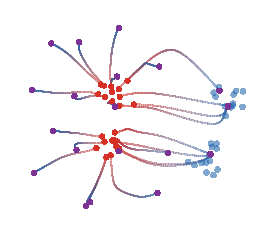
\includegraphics[width=.34\linewidth]{figures/generative-drifting-model-trajectories/unnormalized-trajectories.pdf} &
\index{drifting!model}% strictindex
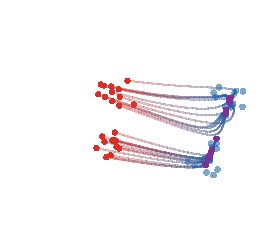
\includegraphics[width=.34\linewidth]{figures/generative-drifting-model-trajectories/normalized-trajectories.pdf}
\\[-.1em]
\small unnormalized Gaussian drift & \small normalized Gaussian drift
\index{self-corrected field}% strictindex
\end{tabular}
\caption{\emph{Two schematic Gaussian-kernel drifting trajectories for a small particle generator.} Both panels use attraction-minus-weighted-self fields. The left uses unnormalized Gaussian averages; the right uses normalized Gaussian mean-shift averages. Their target and self bandwidths, self weights, integration horizons and step sizes differ, and both simulations cap the instantaneous speed. The display compares two tuned constructions rather than a controlled ablation of self-repulsion.}
\label{fig:generative-drifting-model-trajectories}
\end{figure}

\subsection{Evolution in Depth of Transformers}
\label{sec-transformer-depth-evolution}
\index{transformer}% strictindex
\index{depth evolution}% strictindex

Deep residual architectures can be read as time discretizations of ODEs or PDEs. For transformers, the transported objects are token measures and the velocity is induced by attention.
\index{attention}% strictindex
\index{token measure}% strictindex

\paragraph{Tokens and mean-field attention.}
Transformers were introduced as sequence-to-sequence architectures driven by self-attention~\citep{Vaswani2017Attention} and have become central to language and vision models~\citep{Brown2020LanguageModels,Dosovitskiy2021Image}. After tokenization, embedding and any positional encoding, an input is represented by vectors \(x_1,\ldots,x_n\in\RR^d\), called \emph{tokens}. A transformer manipulates these vectors through a succession of attention, tokenwise neural-network and normalization layers. Attention is the principal mixing operation: it associates with each token a data-dependent weighted average of the value vectors carried by the full token population.
\index{positional encoding}% strictindex

Consider one attention head with parameters \(\theta=(Q,K,V)\), suppressing biases and the final output projection. Here \(Q,K\in\RR^{r\times d}\) are the query and key matrices and \(V\in\RR^{d\times d}\) is the value matrix. Thus \(Qx_i\) is the query carried by token \(i\), while \(Kx_j\) and \(Vx_j\) are the key and value carried by token \(j\). In the non-causal, unmasked setting used here, its discrete output is
\begin{equation}\label{eq-discrete-self-attention}
	\operatorname{Att}^{(n)}_\theta(x_1,\ldots,x_n)_i
	\eqdef
	\sum_{j=1}^n a_{i,j}(x_1,\ldots,x_n)Vx_j,
	\qquad
	a_{i,j}(x_1,\ldots,x_n)
	\eqdef
	\frac{\exp(\dotp{Qx_i}{Kx_j})}
	{\sum_{\ell=1}^n\exp(\dotp{Qx_i}{Kx_\ell})},
\end{equation}
Thus every query token may attend to every key token. Causal attention instead masks future indices; the resulting order dependence is deliberately omitted here. The conventional factor \(1/\sqrt r\) in the score can be absorbed into \(Q\) or \(K\).
\index{attention!non-causal}% strictindex
\index{attention!causal}% strictindex
\index{attention!masking}% strictindex

The map~\eqref{eq-discrete-self-attention} is permutation equivariant. Indeed, if \(\sigma\) is a permutation and \(x_i^\sigma=x_{\sigma(i)}\), reindexing the denominator gives \(a_{i,j}(x_1^\sigma,\ldots,x_n^\sigma)=a_{\sigma(i),\sigma(j)}(x_1,\ldots,x_n)\), and therefore
\[
	\operatorname{Att}^{(n)}_\theta(x_1^\sigma,\ldots,x_n^\sigma)_i
	=
	\operatorname{Att}^{(n)}_\theta(x_1,\ldots,x_n)_{\sigma(i)}.
\]
Relabeling the input tokens therefore only relabels the outputs. This statement concerns the already encoded token vectors: a causal mask or external position labels break this plain symmetry unless the position is retained as part of the token state. In the unmasked setting, permutation equivariance suggests replacing the ordered tuple by its empirical measure \(\al=n^{-1}\sum_{i=1}^n\de_{x_i}\).
\index{permutation!equivariance}% strictindex
\index{empirical!token measure}% strictindex


\begin{defn}[Mean-field attention map]\label{def-mean-field-attention-map}
\index{attention!mean-field map}% strictindex
	Fix \(p\geq1\), let $Q,K\in\RR^{r\times d}$ and $V\in\RR^{d\times d}$, write \(\theta=(Q,K,V)\), and let \(\al\in\Pp_p(\RR^d)\). Assume that, for \(\al\)-almost every \(x\),
	\[
		0<\int e^{\dotp{Qx}{Kz}}\,\d\al(z)<+\infty
		\qandq
		\int e^{\dotp{Qx}{Kz}}\norm{Vz}\,\d\al(z)<+\infty.
	\]
	The \emph{mean-field attention field} is
	\begin{equation}\label{eq-mean-field-attention}
		\Gamma_\theta[\al](x)
		\eqdef
		\frac{\int e^{\dotp{Qx}{Kz}}Vz\,\d\al(z)}
		{\int e^{\dotp{Qx}{Kz}}\,\d\al(z)}
	\end{equation}
	and, whenever \(\Gamma_\theta[\al]\in L^p(\al)\), the induced attention map on measures is
	\[
		\operatorname{Att}_\theta(\al)
		\eqdef
		(\Gamma_\theta[\al])_\sharp\al.
	\]
\end{defn}

These assumptions are automatic on compact supports. For $\alpha=n^{-1}\sum_i\delta_{x_i}$, one has $\Gamma_\theta[\alpha](x_i)=\operatorname{Att}^{(n)}_\theta(x_1,\ldots,x_n)_i$: the measure formulation is an exact rewriting, not an approximation. A many-token limit requires additional stability and compactness assumptions.

Here our principal limit concerns depth: the number $T$ of residual attention layers grows while each layer makes an update of size $1/T$, as in continuous-depth neural networks~\citep{Chen2018NeuralODE}. This is distinct from increasing the token count $n$. The whole current token law normalizes the attention weights, making the induced velocity nonlinear and context dependent. Related continuous-depth and Sinkhorn-normalized dynamics are studied in~\citet{Sander2022Sinkformers,Castin2025DynamicsTransformers}.
\index{continuous-depth neural network}% strictindex
\index{empirical!context}% strictindex
\index{attention!operator}% strictindex
\index{infinite-depth limit}% strictindex
\index{token limit}% strictindex
\index{transformer}% strictindex
\index{mean-field limit}% strictindex
\index{continuous!depth}% strictindex

We focus on the non-causal single-head mechanism of~\eqref{eq-discrete-self-attention}, ignoring MLP layers, layer normalization and masking. This stripped-down framework isolates the transport structure of a residual attention block.
\index{attention!single-head}% strictindex
\index{layer normalization}% strictindex
\index{causality}% strictindex
\index{masking}% strictindex
\index{transformer}% strictindex

\paragraph{Attention as a context-dependent velocity.}
\index{attention}% strictindex
\index{velocity field}% strictindex

We retain the notation \(\theta=(Q,K,V)\) and \(\Gamma_\theta\) of Definition~\ref{def-mean-field-attention-map}. Whereas~\eqref{eq-discrete-self-attention} replaces a token by its attention output, a residual block adds this output through a skip connection. With residual scale \(1/T\), it acts as
\begin{equation}\label{eq-transformer-residual-attention-step}
	x_i
	\longmapsto
	x_i+\frac1T\operatorname{Att}^{(n)}_\theta(x_1,\ldots,x_n)_i
	=
	x_i+\frac1T
	\sum_{j=1}^n
	\frac{e^{\dotp{Qx_i}{Kx_j}}Vx_j}
	{\sum_{\ell=1}^n e^{\dotp{Qx_i}{Kx_\ell}}}.
\end{equation}
The attention output is therefore interpreted as a context-dependent velocity, and the skip connection performs one explicit Euler step along this field.
\index{skip connection}% strictindex
\index{explicit Euler scheme}% strictindex

\paragraph{Token measure evolution.}
\index{residual attention}% strictindex
\index{in-context map}% strictindex
\index{token measure}% strictindex

Let \(x_i^{(\ell)}\) be token \(i\) after layer \(\ell\), and let \(\al^{(\ell)}=n^{-1}\sum_i\de_{x_i^{(\ell)}}\) be the corresponding empirical law. With \(\tau=1/T\), equation~\eqref{eq-transformer-residual-attention-step} is exactly
\begin{equation}\label{eq-transformer-residual-measure-step}
	\al^{(\ell+1)}
	=
	\left(
		\Id+\tau\Gamma_{\theta^{(\ell)}}[\al^{(\ell)}]
	\right)_\sharp
	\al^{(\ell)},
	\qquad
	\ell=0,\ldots,T-1.
\end{equation}
Unlike the non-residual map \(\operatorname{Att}_\theta\) of Definition~\ref{def-mean-field-attention-map}, this update keeps each current token and adds a small attention displacement.
\index{empirical!measure}% strictindex
\index{transformer}% strictindex
Set \(t_\ell=\ell/T\) and suppose that \(\theta^{(\ell)}\) samples a sufficiently regular depth-dependent path \(t\mapsto\theta_t\). As \(T\to+\infty\), a time interpolation of~\eqref{eq-transformer-residual-measure-step} converges formally to the conservation equation
\begin{equation}\label{eq-transformer-mean-field-pde}
	\partial_t\al_t
	+
	\diverg\!\left(\al_t\Gamma_{\theta_t}[\al_t]\right)
	=
	0.
\end{equation}



\paragraph{$L^2$ attention and mean shift.}
\index{L2 self-attention@$L^2$ self-attention}% strictindex
\index{mean-shift PDE}% strictindex
\index{kernel!regression}% strictindex
\index{attention!Gaussian kernel}% strictindex
\index{mean shift}% strictindex

A particularly geometric variant replaces the dot-product score \(\dotp{Qx}{Ky}\) by a negative squared Euclidean score \(s_\epsilon(x,y)=-\norm{x-y}^2/(2\epsilon)\). Take, for simplicity, the same token space for queries, keys and values, and set
\[
	K_\epsilon(x,y)=\exp(-\norm{x-y}^2/(2\epsilon)),
	\qquad
	\rho_\epsilon[\alpha](x)=\int K_\epsilon(x,y)\d\alpha(y),
	\qquad
	m_\epsilon[\alpha](x)
	=
	\frac{\int yK_\epsilon(x,y)\d\alpha(y)}
	     {\rho_\epsilon[\alpha](x)}.
\]
The map $x\mapsto m_\epsilon[\alpha](x)$ is exactly Gaussian-kernel attention, i.e.\ normalized kernel regression over tokens; such $L^2$ or Gaussian-kernel scores are used explicitly in transformer variants motivated by Lipschitz control and projection-free attention~\citep{KimPapamakariosMnih2020L2SelfAttention,KunduGhoshGhoshHonavar2026GaussianKernelAttention}. Classical mean shift, however, uses the displacement from the current point to this local barycenter. This gives
\index{L2 attention@$L^2$ attention}% strictindex
\index{projection-free attention}% strictindex
\begin{equation}\label{eq-l2-attention-mean-shift}
	M_\epsilon[\alpha](x)
	\eqdef
	m_\epsilon[\alpha](x)-x
	=
	\frac{\int (y-x)K_\epsilon(x,y)\d\alpha(y)}
	     {\rho_\epsilon[\alpha](x)}
	=
	\epsilon\nabla\log\rho_\epsilon[\alpha](x)
\end{equation}
and, when $\alpha$ is empirical, $\rho_\epsilon[\alpha]$ is a Gaussian kernel density estimate up to normalization. Thus \(M_\epsilon[\alpha]\) is the classical Gaussian mean-shift vector~\citep{FukunagaHostetler1975,Cheng1995MeanShift,ComaniciuMeer2002MeanShift}. If the data measure $\alpha$ is frozen, the update $x\leftarrow m_\epsilon[\alpha](x)$ is the usual mode-seeking mean-shift iteration. If instead all support points move and the empirical measure is recomputed after every step, one obtains the self-consistent, or \emph{blurring}, mean-shift process~\citep{Chen2015BlurringMeanShift}. Its damped update is
\index{mean shift!blurring}% strictindex
\index{kernel!density estimate}% strictindex
\index{mean shift!vector}% strictindex
\[
	x_i^{(\ell+1)}
	=
	(1-\tau)x_i^{(\ell)}+\tau m_\epsilon[\alpha^{(\ell)}](x_i^{(\ell)})
	=
	x_i^{(\ell)}+\tau M_\epsilon[\alpha^{(\ell)}](x_i^{(\ell)})
\]
which is an explicit Euler step of the continuous-time mean-shift equation
\[
	\partial_t\alpha_t+\diverg\bigl(\alpha_tM_\epsilon[\alpha_t]\bigr)=0.
\]
For $\tau=1$ this is discrete blurring mean shift; for small $\tau$ it approximates a transport PDE that moves each token uphill along the log of the smoothed token density. This distinction between the raw barycentric attention output $m_\epsilon$ and the velocity $M_\epsilon=m_\epsilon-\Id$ is important: adding $m_\epsilon$ directly as a residual would produce a different drift. The mean-shift form isolates a purely metric attention mechanism from the learned bilinear geometry of $\dotp{Qx}{Ky}$.
\index{mean shift!iteration}% strictindex
\index{barycentric!attention}% strictindex

\begin{rem}[Consensus for blurring mean shift]\label{rem-mean-shift-consensus}
\index{opinion dynamics}% strictindex
\index{consensus}% strictindex
\index{clustering}% strictindex
\index{bounded confidence}% strictindex
\index{mean shift!blurring}% strictindex
The self-consistent mean-shift equation is a continuum consensus model. If $\alpha_0$ is compactly supported and the interaction kernel is positive and Lipschitz on the convex hull of its support, that hull is forward invariant and the normalized averaging kernels share a uniform positive fraction of mass. This common contribution contracts each directional width of the moving support, and hence its diameter. Under the corresponding characteristic well-posedness assumptions, it yields exponential contraction of the support diameter and convergence of $\alpha_t$ in every $\Wass_p$, $1\leq p<+\infty$, to a Dirac mass; see~\citet{HegselmannKrause2002OpinionDynamics,Chen2015BlurringMeanShift,MotschTadmor2014Heterophilious} and the finite-agent and Eulerian consensus analyses in~\citet{BlondelHendrickxTsitsiklis2009Krause,CanutoFagnaniTilli2012EulerianKrause}. Without strict positivity, consensus is no longer guaranteed: bounded-confidence kernels can disconnect the interaction graph and produce several clusters instead of one consensus point. Moreover, because the normalized interactions are generally asymmetric, the limiting point need not be the initial barycenter.
\end{rem}

Figure~\ref{fig:generative-mean-shift-pde} visualizes the long transient before this eventual consensus: particles climb the current smoothed density while the density itself sharpens.

\begin{figure}[htbp]
\centering
\begin{tabular}{@{}c@{\hspace{.5em}}c@{}}
\raisebox{-.5\height}{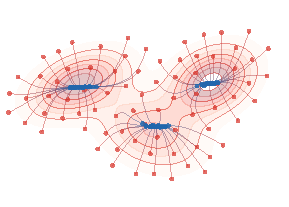
\includegraphics[width=.39\linewidth]{figures/generative-mean-shift-pde/trajectories.pdf}} &
\begin{tabular}{@{}cc@{}}
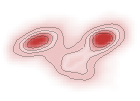
\includegraphics[width=.185\linewidth]{figures/generative-mean-shift-pde/snapshot-1.pdf} &
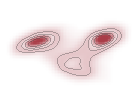
\includegraphics[width=.185\linewidth]{figures/generative-mean-shift-pde/snapshot-2.pdf} \\
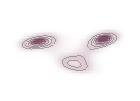
\includegraphics[width=.185\linewidth]{figures/generative-mean-shift-pde/snapshot-3.pdf} &
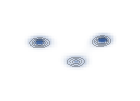
\includegraphics[width=.185\linewidth]{figures/generative-mean-shift-pde/snapshot-4.pdf}
\end{tabular}
\\[-.2em]
\small trajectories on the initial density & \small later density snapshots
\end{tabular}
\caption{\emph{Continuous-time mean shift for a densely sampled three-Gaussian mixture.} Left: initial density level sets, in red, and representative particle paths of $\dot x=M_\epsilon[\alpha_t](x)$, colored from red to blue. Right: four later kernel-density renderings of $\alpha_t$ at increasing times, with the same red-to-blue time palette; the initial density is omitted because it is shown on the left. The snapshots show the long multimodal transient before the globally positive Gaussian interactions drive the cloud toward the one-point consensus described in Remark~\ref{rem-mean-shift-consensus}.}
\label{fig:generative-mean-shift-pde}
\end{figure}
\index{kernel!Gaussian}% strictindex
\index{kernel!regression}% strictindex
\index{transport!PDE}% strictindex

\paragraph{Gradient structure and limitations.}
\index{gradient!structure}% strictindex

When the token space has dimension $d$ and the query/key space has dimension $r$, take $Q,K\in\RR^{r\times d}$ and $V\in\RR^{d\times d}$. Assume compact token support, or sufficient exponential-moment bounds to justify differentiation under the integrals below. If $V=Q^\top K$, the field $\Gamma_\theta[\alpha]$ is a gradient vector field in the token variable. Indeed, define the log-partition potential
\[
	\Phi_\alpha(x)
	=
	\int \exp(\dotp{Qx}{Ky})\d\alpha(y),
	\qquad
	U_\alpha(x)=\log\Phi_\alpha(x).
\]
Then
\[
	\nabla_x U_\alpha(x)
	=
	\frac{\int Q^\top K y\,\exp(\dotp{Qx}{Ky})\d\alpha(y)}
	     {\int \exp(\dotp{Qx}{Kz})\d\alpha(z)}
	=
	\Gamma_\theta[\alpha](x).
\]
This proves only that the velocity is an instantaneous gradient in $x$; it does not by itself identify a Wasserstein energy. Indeed, the natural scalar candidate $f_{\rm att}(\alpha)=\int U_\alpha(x)\,\d\alpha(x)$ has first variation
\[
	\delta f_{\rm att}(\alpha)(z)
	=
	U_\alpha(z)
	+
	\int
	\frac{\exp(\dotp{Qx}{Kz})}{\Phi_\alpha(x)}
	\,\d\alpha(x),
\]
up to an additive constant. The second term is the response of every query normalization to a perturbation of the key distribution, and its spatial gradient is absent from $\Gamma_\theta[\alpha]$. Thus, without additional symmetry or integrability conditions, the displayed attention PDE is a transportation dynamics rather than the Wasserstein gradient flow of this fixed scalar functional. Special variants recover additional structure: Sinkhorn attention can be interpreted through doubly stochastic normalization and Wasserstein-type gradient flows~\citep{Sander2022Sinkformers,Castin2025DynamicsTransformers}, while layer normalization leads naturally to dynamics on the sphere and to modified metrics. The key open difficulty for the present viewpoint is training: after the architecture has been rewritten as a controlled transport equation, learning corresponds to optimizing the time-dependent parameters $(\theta_t)_t$ rather than merely analyzing the forward PDE for fixed parameters.
\index{transformer}% strictindex
\index{doubly stochastic normalization}% strictindex
\index{transport!equation}% strictindex
\index{controlled transport}% strictindex
\index{first variation}% strictindex
\index{layer normalization}% strictindex
\index{Wasserstein!gradient}% strictindex
\index{gradient!flow}% strictindex
\index{Wasserstein!gradient flow}% strictindex
\index{attention}% strictindex

\subsection{Flows over the Gaussian Manifold}
\label{sec-gaussian-closure-transport-dynamics}
\index{Gaussian!manifold}% strictindex

Gaussian measures provide a useful testing ground for the preceding dynamics. They are not invariant under a general Wasserstein gradient flow: a nonlinear velocity usually creates non-Gaussian densities immediately. The useful substitute is to either identify affine velocities, which exactly preserve Gaussianity, or to project the dynamics onto the Gaussian manifold. In both cases the measure PDE reduces to matrix ODEs for the mean and covariance. This viewpoint is emphasized in the survey~\citep{Peyre2026OptimalDiffusionTransports} and is useful for comparing diffusion paths, Wasserstein gradient flows, drifting fields and transformer-type dynamics.
\index{affine!closure}% strictindex
\index{drifting!field}% strictindex
\index{Wasserstein!gradient}% strictindex
\index{gradient!flow}% strictindex
\index{transformer}% strictindex
\index{Wasserstein!gradient flow}% strictindex
\index{Gaussian!manifold}% strictindex
\index{Gaussian!measure}% strictindex

For constrained gradient flows on this family, the covariance equation is the finite-dimensional Bures--Wasserstein gradient flow on positive definite matrices. This restricted metric is the same in both settings, but exact ambient preservation and deliberate projection onto the submanifold remain distinct claims. Figure~\ref{fig:gradflow-gaussian-closure} first compares two illustrative Gaussian paths from a source \(\alpha_0\) to a target \(\gamma\); the exact ambient equations admitting Gaussian solutions for specified energies \(f(\alpha)\) are catalogued afterwards in Proposition~\ref{prop-centered-gaussian-covariance-catalogue}.
\index{Gaussian!submanifold}% strictindex
\index{affine!gradient}% strictindex
\index{Bures!Wasserstein geometry}% strictindex
\index{Wasserstein!gradient}% strictindex
\index{Gaussian!closure}% strictindex
\index{gradient!flow}% strictindex

\begin{figure}[ht]
\centering
\begin{tabular}{@{}c@{\hspace{1.5em}}c@{}}
\small $\Wass_2$ geodesic & \small drifting closure \\[-.15em]
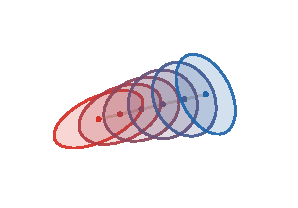
\includegraphics[width=.30\linewidth]{figures/gradflow-gaussian-closure/ot-ellipses.pdf} &
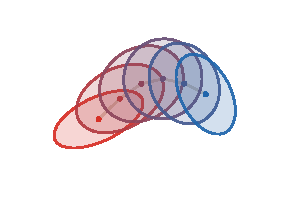
\includegraphics[width=.30\linewidth]{figures/gradflow-gaussian-closure/drifting-ellipses.pdf}
\end{tabular}
\caption{\emph{Two Gaussian paths from a red source $\alpha_0$ to a blue target $\gamma=\Gaussian(\bar m,\bar\Sigma)$.} The left panel is the constant-speed $\Wass_2$ geodesic minimizing the Benamou--Brenier action. The right panel is a prescribed non-variational drifting flow with an affine Gaussian-preserving velocity: its mean follows a curved path while its covariance reaches the same endpoint.}
\index{moment matching}% strictindex
\index{Gaussian!closure}% strictindex
\index{velocity field}% strictindex
\label{fig:gradflow-gaussian-closure}
\end{figure}

\paragraph{Gaussianity preservation.}
\index{Gaussian!preservation}% strictindex

The first question is invariance: one wants a simple criterion ensuring that the continuity equation does not leave the finite-dimensional Gaussian family.
\index{continuity equation}% strictindex


\begin{prop}[Affine velocities preserve Gaussianity]\label{prop-gaussian-affine-closure}
\index{affine!closure}% strictindex
	Let $\alpha_0=\Gaussian(m_0,\Sigma_0)$, with $\Sigma_0\succ0$. Let $b_t\in\RR^d$ and $A_t\in\RR^{d\times d}$ be locally integrable on a time interval, and let $(m_t,\Sigma_t)$ solve
	\[
		\dot m_t=b_t,
		\qquad
		\dot\Sigma_t=A_t\Sigma_t+\Sigma_tA_t^\top,
		\qquad
		(m_{t=0},\Sigma_{t=0})=(m_0,\Sigma_0).
	\]
	Then, as long as this matrix ODE is defined, $\Sigma_t\succ0$ and
	\[
		\alpha_t=\Gaussian(m_t,\Sigma_t)
	\]
	is the solution of the continuity equation
	\[
		\partial_t\alpha_t+\diverg(\alpha_t v_t)=0,
		\qquad
		v_t(x)=b_t+A_t(x-m_t).
	\]
	In particular, if a smooth functional $f$ has a Wasserstein gradient on Gaussian measures of the affine form
	\[
		\Wgrad f(\Gaussian(m,\Sigma))(x)
		=
		b_f(m,\Sigma)+A_f(m,\Sigma)(x-m),
	\]
	with $A_f(m,\Sigma)$ symmetric, then the displayed moment ODE below produces a Gaussian distributional solution of the full Wasserstein gradient-flow equation for $f$:
	\[
		\dot m_t=h_f(m_t,\Sigma_t),
		\qquad
		\dot\Sigma_t=H_f(m_t,\Sigma_t),
	\]
	where
	\[
		h_f(m,\Sigma)=-b_f(m,\Sigma),
		\qquad
		H_f(m,\Sigma)
		=
		-\bigl(A_f(m,\Sigma)\Sigma+\Sigma A_f(m,\Sigma)\bigr).
	\]
	Conversely, fix a non-degenerate Gaussian \(\Gaussian(m,\Sigma)\). Suppose that a finite-energy Wasserstein tangent field \(V_{m,\Sigma}\) is represented by a gradient in \(L^2(\Gaussian(m,\Sigma))\) and is tangent to the Gaussian manifold at this Gaussian. Then there exist \(b(m,\Sigma)\) and a symmetric matrix \(A(m,\Sigma)\) such that
	\[
		V_{m,\Sigma}(x)=b(m,\Sigma)+A(m,\Sigma)(x-m)
		\qquad
		\Gaussian(m,\Sigma)\text{-a.e.}
	\]
	Consequently, under the same smoothness assumptions, if the Wasserstein gradient flow of a functional preserves the Gaussian family for all non-degenerate Gaussian initial data, then \(\Wgrad f(\Gaussian(m,\Sigma))\) is affine on each Gaussian. Without the Wasserstein gradient representative, this converse is false because one may add velocity fields with zero \(\Gaussian(m,\Sigma)\)-weighted divergence.
\index{affine!closure}% strictindex
\index{Wasserstein!gradient}% strictindex
\index{Gaussian!manifold}% strictindex
\index{divergence-free field}% strictindex

	Finally, any smooth Gaussian curve with positive definite covariance can be generated by an affine velocity. If one wants the velocity to be a Wasserstein tangent gradient, one chooses the unique symmetric solution of the Lyapunov equation
\index{affine!closure}% strictindex
\index{Lyapunov equation}% strictindex
	\[
		A_t\Sigma_t+\Sigma_t A_t=\dot\Sigma_t.
	\]
\end{prop}

\begin{proof}
	Let \(X_t\) follow the characteristic ODE \(\dot X_t=b_t+A_t(X_t-m_t)\) with \(X_0\sim\Gaussian(m_0,\Sigma_0)\). Since \(\dot m_t=b_t\), the centered variable \(\tilde X_t=X_t-m_t\) solves the homogeneous linear ODE \(\dot{\tilde X}_t=A_t\tilde X_t\). If \(\Phi_t\) is the fundamental matrix \(\dot\Phi_t=A_t\Phi_t\), \(\Phi_{t=0}=\Id\), then
	\[
		X_t=m_t+\Phi_t(X_0-m_0),
		\qquad
		\Sigma_t=\Phi_t\Sigma_0\Phi_t^\top.
	\]
	Hence \(X_t\) is Gaussian and \(\Sigma_t\succ0\), and
\index{random variable}% strictindex
	\[
		\dot\Sigma_t
		=
		\frac{\d}{\d t}\EE\bigl(\tilde X_t\tilde X_t^\top\bigr)
		=
		A_t\Sigma_t+\Sigma_t A_t^\top.
	\]
	This proves Gaussian preservation and the moment ODE\@. The Wasserstein gradient-flow statement follows by inserting the descent velocity $v_t=-\Wgrad f(\alpha_t)$.
\index{Wasserstein!gradient}% strictindex

	For the converse, fix $\alpha=\Gaussian(m,\Sigma)$ and denote its density by $\rho$. Tangency to the Gaussian manifold means that the density variation $-\diverg(\rho V)$ is generated by some moment variation $(\dot m,\dot\Sigma)$, with $\dot\Sigma$ symmetric. Set $b=\dot m$, and let $A=A^\top$ be the unique solution of
	\(A\Sigma+\Sigma A=\dot\Sigma\).
	By the first part of the proposition, the affine gradient field $V_0(x)=b+A(x-m)$ generates exactly the same infinitesimal Gaussian variation. Hence
	\(\diverg\bigl(\rho(V-V_0)\bigr)=0\)
	in the distributional sense. Both $V$ and $V_0$ belong to the $L^2(\alpha)$ closure of gradient fields. The weighted Helmholtz decomposition therefore makes $V-V_0$ simultaneously a tangent gradient and orthogonal to every tangent gradient, so $V=V_0$ in $L^2(\alpha)$. Equivalently, for a smooth representative $V-V_0=\nabla\psi$, integration by parts gives $\int\norm{\nabla\psi}^2\d\alpha=0$. This proves that the Wasserstein tangent representative is affine. The qualification is essential: without selecting the gradient representative, one can add a nonzero field with zero $\alpha$-weighted divergence without changing the Gaussian curve.
\index{Helmholtz decomposition}% strictindex

	For a prescribed smooth Gaussian curve, set $b_t=\dot m_t$ and choose any matrix $A_t$ satisfying $A_t\Sigma_t+\Sigma_tA_t^\top=\dot\Sigma_t$. Since $\Sigma_t$ is positive definite, the Lyapunov map $A\mapsto A\Sigma_t+\Sigma_t A$ is invertible on symmetric matrices, which gives the unique symmetric choice when a gradient velocity is required. In that case $v_t$ is the gradient of the quadratic potential $x\mapsto \dotp{b_t}{x}+\dotp{A_t(x-m_t)}{x-m_t}/2$.
\index{quadratic!potential}% strictindex
\index{gradient!velocity}% strictindex
\end{proof}

\paragraph{Gaussian-preserving gradient flows.}
\index{Gaussian!preservation}% strictindex
\index{gradient!flow}% strictindex

We now instantiate the affine-gradient viewpoint by tracking functionals whose full Wasserstein gradient is affine on Gaussian inputs. The catalogue below gives exact Gaussian solutions of the ambient Wasserstein equations, not projected or constrained flows. Whenever the ambient equation is unique in the solution class under consideration, this solution is the selected Wasserstein gradient flow and proves invariance of the Gaussian family; without such a uniqueness theorem, it still proves existence of a Gaussian distributional solution, but not invariance of every weak solution.
\index{Wasserstein!gradient}% strictindex
\index{moment functional}% strictindex

\begin{prop}[Gaussian closure catalogue]\label{prop-centered-gaussian-covariance-catalogue}
\index{Gaussian!covariance}% strictindex
\index{Gaussian!mean}% strictindex
\index{Gaussian!manifold}% strictindex
	In the moment-functional row, assume $g$ is continuously differentiable in $(m,\Sigma)$. Let \(\gamma=\Gaussian(\bar m,\bar\Sigma)\) on \(\RR^d\), with \(\bar\Sigma\succ0\), and let the initial condition be \(\alpha_0=\Gaussian(m_0,\Sigma_0)\), with \(\Sigma_0\succ0\). For each functional displayed below, evaluating its ambient Wasserstein gradient on a Gaussian gives an affine field. Consequently, as long as the following finite-dimensional ODE exists and \(\Sigma_t\succ0\),
	\[
		\alpha_t=\Gaussian(m_t,\Sigma_t)
	\]
	is an exact distributional solution of the corresponding ambient gradient-flow PDE, and its mean and covariance satisfy
	\[
		\dot{m}_t=h(m_t,\Sigma_t),
		\qquad
		\dot{\Sigma}_t=H(m_t,\Sigma_t).
	\]
	Write \(\delta_m=m-\bar m\), \(A=\bar\Sigma^{-1}\), and
	\[
		M_{\Sigma,\bar\Sigma}
		\eqdef
		\Sigma^{-1/2}\bigl(\Sigma^{1/2}\bar\Sigma\Sigma^{1/2}\bigr)^{1/2}\Sigma^{-1/2}.
	\]
	The relative Fisher information, used only as an energy in this catalogue, is
	\[
		\mathcal I(\alpha|\gamma)
		=
		\int \left|\nabla\log\frac{\rho(x)}{\rho_\gamma(x)}\right|^2\rho(x)\,\d x
		=
		\int
		\left|\nabla\log\rho(x)+A(x-\bar m)\right|^2\rho(x)\,\d x
		\qquad(\alpha=\rho\,\d x),
	\]
	where $\rho$ is smooth and positive and $\rho_\gamma$ is the density of $\gamma$. For the MMD row, set $R=\Sigma+m\,m^\top-\bar\Sigma-\bar m\,\bar m^\top$.
	With the normalizations displayed in the first column, the mean vector field \(h\) and covariance vector field \(H\) are listed in the following table. If that PDE is unique in the selected solution class, this Gaussian solution is the Wasserstein flow from \(\alpha_0\). Gradients with respect to \(\Sigma\) are symmetric Frobenius gradients on the cone of covariance matrices.
	\index{maximum mean discrepancy}% strictindex
		\begin{center}
		\begingroup
		\small
		\renewcommand{\arraystretch}{1.55}
		\begin{tabularx}{\linewidth}{>{\raggedright\arraybackslash}p{.42\linewidth}>{\centering\arraybackslash}p{.18\linewidth}>{\raggedright\arraybackslash}X}
			\hline
			Functional \(f(\alpha)\) & \(h(m,\Sigma)\) & \(H(m,\Sigma)\) \\
			\hline
			\(g(m_\alpha,\Sigma_\alpha)\)
			&
			\(-\nabla_m g\)
			&
			\(-2(\Sigma\nabla_\Sigma g+\nabla_\Sigma g\,\Sigma)\)
			\\
			\(\displaystyle \int\Bigl(\frac12x^\top Bx+\dotp{\ell}{x}\Bigr)\d\alpha(x)\), \(B=B^\top\)
			&
			\(-(B m+\ell)\)
			&
			\(-(\Sigma B+B\Sigma)\)
			\\
			\(\displaystyle \frac14\iint (x-y)^\top G(x-y)\d\alpha(x)\d\alpha(y)\), \(G=G^\top\)
			&
			\(0\)
			&
			\(-(\Sigma G+G\Sigma)\)
			\\
			\(\KL(\alpha|\gamma)\)
			&
			\(-A\delta_m\)
			&
			\(2\Id-\Sigma A-A\Sigma\)
			\\
			\(\mathcal I(\alpha|\gamma)\)
			&
			\(-2A^2\delta_m\)
			&
			\(4\Sigma^{-1}-2\Sigma A^2-2A^2\Sigma\)
			\\
			\(\Wass_2^2(\alpha,\gamma)\)
			&
			\(-2\delta_m\)
			&
			\(2(M_{\Sigma,\bar\Sigma}\Sigma+\Sigma M_{\Sigma,\bar\Sigma}-2\Sigma)\)
			\\
			\(\MMD_k^2(\alpha,\gamma)\), \(k(x,y)=\dotp{x}{y}^2\)
			&
			\(-4R m\)
			&
			\(-4(\Sigma R+R\Sigma)\)
			\\
			\hline
		\end{tabularx}
		\endgroup
		\end{center}
\end{prop}

\begin{proof}
	For the moment-functional row, the formula is exact on the full Wasserstein space. Indeed, write $m_\alpha=\int x\,\d\alpha(x)$ and $\Sigma_\alpha=\int (x-m_\alpha)(x-m_\alpha)^\top\d\alpha(x)$. If \(\eta\) is a signed perturbation with zero total mass, then $\d m_\alpha[\eta]=\int x\,\d\eta(x)$ and $\d\Sigma_\alpha[\eta]=\int (x-m_\alpha)(x-m_\alpha)^\top\d\eta(x)$. Thus, up to an irrelevant additive constant, the first variation is $\delta f(\alpha)(x)=\dotp{\nabla_m g}{x}+\dotp{\nabla_\Sigma g}{(x-m_\alpha)(x-m_\alpha)^\top}$,
	and its spatial gradient is the affine field
	\[
		\nabla_x\delta f(\alpha)(x)
		=
		\nabla_m g+2\nabla_\Sigma g\,(x-m_\alpha).
	\]
	Consequently the full Wasserstein descent velocity is affine, and Proposition~\ref{prop-gaussian-affine-closure} gives the displayed moment equations.
\index{moment functional}% strictindex
\index{first variation}% strictindex

	For the quadratic potential row, the ambient first variation is
	\[
		\delta f(\alpha)(x)=\frac12x^\top Bx+\dotp{\ell}{x},
		\qquad
		\nabla_x\delta f(\alpha)(x)=B m+\ell+B(x-m),
	\]
	which gives the displayed affine velocity. For the quadratic interaction row, the ambient first variation is $\delta f(\alpha)(x)=\frac12\int (x-y)^\top G(x-y)\d\alpha(y)$, with $\nabla_x\delta f(\alpha)(x)=G(x-m_\alpha)$.
	These first variations are quadratic in \(x\), hence the affine Gaussian flow coincides with the full Wasserstein gradient flow.
\index{quadratic!potential}% strictindex
\index{energy!interaction}% strictindex
\index{first variation}% strictindex

	For the KL row, write $\alpha=\rho\,\d x$ and let $\rho_\gamma$ denote the density of $\gamma$. The ambient first variation is \(\log(\rho/\rho_\gamma)\) up to an additive constant. If \(\alpha=\Gaussian(m,\Sigma)\), then
	\[
		\nabla\log(\rho/\rho_\gamma)(x)
		=
		-\Sigma^{-1}(x-m)+A(x-\bar m),
	\]
	so the descent velocity is
	\(v(x)=-A\delta_m+(\Sigma^{-1}-A)(x-m)\).
	Proposition~\ref{prop-gaussian-affine-closure} gives \(h(m,\Sigma)=-A\delta_m\) and \(H(m,\Sigma)=2\Id-\Sigma A-A\Sigma\). For the Fisher row, writing \(u=\log(\rho/\rho_\gamma)\), the ambient first variation of \(\frac12\mathcal I(\alpha|\gamma)\) is, up to constants,
	\[
		-\Delta u-\frac12|\nabla u|^2-\dotp{\nabla u}{\nabla\log\rho_\gamma}.
	\]
	For Gaussian \(\rho\) and Gaussian \(\gamma\), this is quadratic in \(x\). Multiplying by two for \(\mathcal I(\alpha|\gamma)\) gives the descent velocity
	\[
		v(x)=-2A^2\delta_m+2(\Sigma^{-2}-A^2)(x-m).
	\]
	Hence the Wasserstein velocity is affine and the Gaussian family is closed, with the displayed \(h\) and \(H\). Although the ambient Fisher flow is a fourth-order PDE for a generic density, it is therefore an exact finite-dimensional closure in this quadratic-reference case.
\index{Kullback-Leibler@Kullback--Leibler!divergence}% strictindex
\index{Fisher information}% strictindex

	For \(\Wass_2^2(\alpha,\gamma)\), the Brenier map from \(\Gaussian(m,\Sigma)\) to \(\gamma\) is
	\(T(x)=\bar m+M_{\Sigma,\bar\Sigma}(x-m)\).
	The descent velocity for the unhalved squared distance is \(2(T-\Id)\), which gives the mean and covariance equations through Proposition~\ref{prop-gaussian-affine-closure}. For the MMD row, \(k(x,y)=\dotp{x}{y}^2\) identifies the kernel mean embedding with the raw second moment. Thus
	\[
		\MMD_k^2(\alpha,\gamma)
		=
		\norm{\Sigma+m\,m^\top-\bar\Sigma-\bar m\,\bar m^\top}_{\mathrm F}^2
		=
		\norm{R}_{\mathrm F}^2,
	\]
	and the ambient first variation is \(2x^\top R x\), whose descent velocity is \(-4Rx\). This gives \(h(m,\Sigma)=-4R m\) and \(H(m,\Sigma)=-4(\Sigma R+R\Sigma)\).
\index{Brenier!map}% strictindex
\index{Bures!Wasserstein geometry}% strictindex
\index{maximum mean discrepancy}% strictindex
\index{second moment}% strictindex

\end{proof}

\begin{example}[Linear mean-field networks as cross-covariance flows]
\index{flow!cross-covariance}% strictindex
\index{cross-covariance}% strictindex
	Consider the two-layer mean-field model of Section~\ref{sec-wasserstein-flows-mlp}, and take the linear activation $\sigma(s)=s$, so that $\psi((u,v),z)=v\,\dotp{u}{z}$.
\index{two-layer neural network}% strictindex
	We restrict this example to centered neuron laws, $\int (u,v)\d\alpha(u,v)=0$, and write their covariance in blocks as
	\[
		\Sigma_\alpha=
		\begin{pmatrix}
			\Sigma_{u,u}(\alpha) & \Sigma_{u,v}(\alpha)\\
			\Sigma_{v,u}(\alpha) & \Sigma_{v,v}(\alpha)
		\end{pmatrix},
	\]
	and use the lower-left cross-covariance block
	\[
		\Sigma_{v,u}(\alpha)=\int v u^\top\d\alpha(u,v)\in\RR^{d'\times d}.
	\]
	The predictor is therefore the linear map $G_{\alpha_t}(z)=\Sigma_{v,u}(\alpha_t)z$. For the squared Euclidean loss, set $S=\int zz^\top\d\zeta(z,y)$ and $R=\int y z^\top\d\zeta(z,y)$.
\index{second moment}% strictindex
\index{neuron law}% strictindex
	The learning energy of~\eqref{eq-mlp-square-loss-quadratic-linear} is then the covariance functional
	\[
		f(\alpha)=g(\Sigma_\alpha),
		\qquad
		g(\Sigma)
		=
		\frac12\tr\!\big(\Sigma_{v,u}S\Sigma_{u,v}\big)
		-\tr\!\big(R\Sigma_{u,v}\big)
		+\frac12\int\norm{y}^2\d\zeta(z,y).
	\]
	This puts the model exactly in the centered moment-functional row of Proposition~\ref{prop-centered-gaussian-covariance-catalogue}. To see that it recovers the usual particle equation, write $E_\alpha\eqdef \Sigma_{v,u}(\alpha)S-R$. The first variation is $\delta f(\alpha)(u,v)=\dotp{E_\alpha}{v u^\top}=v^\top E_\alpha u$.
\index{first variation}% strictindex
	Hence the particle velocity in parameter space is linear:
	\[
		-\nabla_{(u,v)}\delta f(\alpha)(u,v)
		=
		-\begin{pmatrix}
			0 & E_\alpha^\top \\
			E_\alpha & 0
		\end{pmatrix}
		\begin{pmatrix} u \\ v \end{pmatrix}.
	\]
	Equivalently, at the level of $g$, \(\nabla_\Sigma g=\frac12\begin{pmatrix}0 & E_\alpha^\top\\ E_\alpha & 0\end{pmatrix}\).
	The factor \(1/2\) in the covariance gradient comes from the symmetry of \(\Sigma\): the upper-right block is the transpose of the lower-left block. Substituting this gradient in Proposition~\ref{prop-centered-gaussian-covariance-catalogue} gives
	\[
		\dot m_t=0,
		\qquad
		\dot\Sigma_t=-(\Sigma_t L_t+L_t\Sigma_t),
		\qquad
		L_t=
		\begin{pmatrix}
			0 & E_t^\top\\
			E_t & 0
		\end{pmatrix},
		\qquad
		E_t=\Sigma_{v,u}(\alpha_t)S-R.
	\]
	Thus a centered Gaussian law of neurons remains centered Gaussian, and its coefficient matrix is determined by the cross-covariance block. This block is not generally autonomous by itself: $\dot\Sigma_{v,u}=-E_t\Sigma_{u,u}-\Sigma_{v,v}E_t$ also involves the two diagonal covariance blocks. This exact closure is special to the linear activation; for nonlinear activations, Gaussian closures are usually projections rather than invariant families.
\index{covariance!subblock}% strictindex
\index{neuron law}% strictindex
\index{neuron}% strictindex
\index{Gaussian!closure}% strictindex
\index{affine!closure}% strictindex
\end{example}

\paragraph{One-dimensional case.}
\index{Gaussian!one-dimensional}% strictindex
\index{Gaussian!closure}% strictindex

Fix a Gaussian target $\gamma=\Gaussian(\bar m,\bar\sigma^2)$, with $\bar\sigma>0$, and write $\alpha=\Gaussian(m,\sigma^2)$, with $\sigma>0$. By Proposition~\ref{prop-gaussian-w2-bures}, the parametrization $(m,\sigma)\mapsto\Gaussian(m,\sigma^2)$ identifies the one-dimensional Gaussian family with the open Euclidean half-plane. Hence every Gaussian-preserving functional in Proposition~\ref{prop-centered-gaussian-covariance-catalogue} is represented by the scalar restriction
\[
	g_f(m,\sigma)\eqdef f\bigl(\Gaussian(m,\sigma^2)\bigr).
\]
Set $\delta=m-\bar m$.
The three restrictions used in Figure~\ref{fig:gradflow-gaussian-1d-energy-landscapes} are then
\begin{center}
\begingroup
\small
\renewcommand{\arraystretch}{1.55}
\begin{tabularx}{\linewidth}{>{\raggedright\arraybackslash}p{.34\linewidth}>{\raggedright\arraybackslash}X}
	\hline
	Functional $f(\alpha)$ & Scalar restriction $g_f(m,\sigma)$ \\
	\hline
	$\KL(\alpha\mid\gamma)$
	& $\displaystyle
	\log\frac{\bar\sigma}{\sigma}
	+\frac{\sigma^2+\delta^2}{2\bar\sigma^2}-\frac12$
	\\
	$\Wass_2^2(\alpha,\gamma)$
	& $\displaystyle \delta^2+(\sigma-\bar\sigma)^2$
	\\
	$\mathcal I(\alpha|\gamma)$
	& $\displaystyle
	\frac{\delta^2}{\bar\sigma^4}
	+\frac{(\sigma^2-\bar\sigma^2)^2}{\sigma^2\bar\sigma^4}$
	\\
	\hline
\end{tabularx}
\endgroup
\end{center}
Figure~\ref{fig:gradflow-gaussian-1d-energy-landscapes} compares the three landscapes and their Euclidean gradient-flow trajectories. By Proposition~\ref{prop-centered-gaussian-covariance-catalogue}, these curves give exact Gaussian solutions of the ambient Wasserstein equations rather than the constrained Gaussian approximations introduced next; uniqueness of the ambient solution is a separate analytic issue.
\index{Kullback-Leibler@Kullback--Leibler!divergence}% strictindex
\index{Fisher information!relative}% strictindex
\index{Wasserstein!Gaussian geometry}% strictindex

\begin{figure}[htbp]
\centering
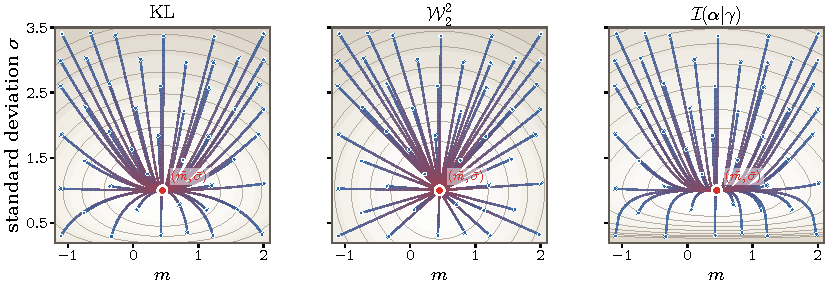
\includegraphics[width=.90\linewidth]{figures/gradflow-gaussian-1d-energy-landscapes/flows-focused.pdf}
\caption{\emph{One-dimensional Gaussian Wasserstein gradient flows in the Euclidean parameter half-plane $(m,\sigma)$.} From left to right, the panels show relative entropy, squared Wasserstein distance, and relative Fisher information. The same $48$ initial parameters are marked in blue; the trajectories progress through violet toward the common target $(\bar m,\bar\sigma)$ in red. Each background uses its own level scale to reveal the geometry of the corresponding energy. The $\Wass_2^2$ trajectories are straight rays, whereas the other functionals bend the evolution of the standard deviation.}
\label{fig:gradflow-gaussian-1d-energy-landscapes}
\end{figure}

\paragraph{Constrained evolution on the Gaussian manifold.}
\index{Gaussian!manifold}% strictindex

The preceding affine-gradient examples have a limited scope: most Wasserstein gradient flows of a functional \(f(\alpha)\) are not closed on the Gaussian manifold. A nonlinear ambient velocity creates higher-order moments immediately, so the exact Gaussian closure usually fails. The constrained viewpoint deliberately replaces the full evolution by its projection onto \(\mathcal G\), forcing the curve to remain Gaussian while keeping the Wasserstein tangent geometry.
\index{affine!closure}% strictindex
\index{Gaussian!projection}% strictindex

Let
\[
	\mathcal G=\{\Gaussian(m,\Sigma):m\in\RR^d,\ \Sigma\succ0\}
\]
be the Gaussian submanifold of $\Pp_2(\RR^d)$. The Wasserstein gradient of a functional constrained to a smooth submanifold $\mathcal M\subset\Pp_2$ is defined as the Riesz representative of the differential restricted to tangent velocities of $\mathcal M$. Formally, under local well-posedness and consistency assumptions, it is the small-step limit of the constrained JKO scheme
\index{Gaussian!submanifold}% strictindex
\index{Wasserstein!gradient}% strictindex
\index{JKO scheme}% strictindex
\[
	\alpha^{(\ell+1)}\in
	\uargmin{\alpha\in\mathcal M}
	\frac{1}{2\tau}\Wass_2^2(\alpha,\alpha^{(\ell)})+f(\alpha).
\]
For $\mathcal M=\mathcal G$, tangent velocities are affine gradient fields $v(x)=b+A(x-m)$ with $A=A^\top$. The constrained gradient is therefore the $L^2(\Gaussian(m,\Sigma))$ projection of the ambient Wasserstein gradient onto this finite-dimensional affine space, whenever the ambient gradient exists.
\index{affine!gradient}% strictindex
\index{Wasserstein!gradient}% strictindex

\begin{prop}[Gaussian-constrained Wasserstein gradients]\label{prop-gaussian-gradient-bullet-list}
	Let $f$ be a smooth functional and assume that its restriction to nondegenerate Gaussian measures can be written as
\index{Gaussian!measure}% strictindex
	\[
		f(\Gaussian(m,\Sigma))=F(m,\Sigma).
	\]
	Then the Wasserstein gradient constrained to the Gaussian family is the affine vector field
\index{Wasserstein!gradient}% strictindex
	\[
		v_F(x)
		=
		\nabla_m F(m,\Sigma)
		+
		2\nabla_\Sigma F(m,\Sigma)(x-m),
	\]
	where $\nabla_\Sigma F$ denotes the symmetric matrix derivative. Equivalently, $v_F$ is the $L^2(\Gaussian(m,\Sigma))$ projection of the ambient Wasserstein gradient onto affine gradient fields, whenever the ambient gradient exists. Hence the gradient descent flow constrained to Gaussian measures satisfies
\index{affine!gradient}% strictindex
\index{Wasserstein!gradient}% strictindex
\index{Gaussian!measure}% strictindex
	\begin{equation}\label{eq-gaussian-wgf-closure}
		\dot m_t=-\nabla_m F(m_t,\Sigma_t),
		\qquad
		\dot\Sigma_t=-2\bigl(\Sigma_t\nabla_\Sigma F(m_t,\Sigma_t)+\nabla_\Sigma F(m_t,\Sigma_t)\Sigma_t\bigr),
	\end{equation}
	and the descent velocity is affine.
\end{prop}

\begin{proof}
	Test the functional along a Gaussian tangent vector, represented by an affine gradient field
\index{affine!gradient}% strictindex
	\(v(x)=b+A(x-m)\)
	with $A$ symmetric. The induced first-order variations are $\dot m=b$ and $\dot\Sigma=A\Sigma+\Sigma A$. Therefore
	\[
		\d F(m,\Sigma)[b,A\Sigma+\Sigma A]
		=
		\dotp{\nabla_m F}{b}
		+
		\tr\!\left(\nabla_\Sigma F(A\Sigma+\Sigma A)\right).
	\]
	Since $A$, $\Sigma$ and $\nabla_\Sigma F$ are symmetric, the second term equals
	\[
		2\,\tr(\nabla_\Sigma F\,A\Sigma)
		=
		\int \dotp{2\nabla_\Sigma F(x-m)}{A(x-m)}\d\Gaussian(m,\Sigma)(x).
	\]
	Together with the mean term, this gives
	\[
		\d F(m,\Sigma)[\dot m,\dot\Sigma]
		=
		\int \dotp{v_F(x)}{v(x)}\d\Gaussian(m,\Sigma)(x)
	\]
	for all affine gradient fields $v$. This identifies the constrained Wasserstein gradient in the induced $L^2(\alpha)$ metric, or equivalently the projection of the ambient gradient when it exists. Substituting the descent velocity $-v_F$ in Proposition~\ref{prop-gaussian-affine-closure} gives~\eqref{eq-gaussian-wgf-closure}.
\index{Wasserstein!gradient}% strictindex
\index{affine!closure}% strictindex
\end{proof}

This proposition is the organizing rule for constrained Gaussian closures: once the scalar energy has been reduced to a function of $(m,\Sigma)$, its constrained Wasserstein gradient is automatically affine and the covariance follows the Bures-type ODE~\eqref{eq-gaussian-wgf-closure}. When the first variation of $f$ is quadratic, this constrained gradient coincides with the full Wasserstein gradient.
\index{first variation}% strictindex
\index{Gaussian!closure}% strictindex


\paragraph{Non-variational Gaussian-preserving flows.}
\index{Gaussian!preservation}% strictindex
\index{Gaussian!preserving flow}% strictindex

The following examples start from prescribed velocities rather than a fixed scalar energy. Their affine structure preserves Gaussianity. Special choices, such as the Ornstein--Uhlenbeck path, also admit a gradient-flow interpretation.
\index{velocity field}% strictindex
\index{Wasserstein!space}% strictindex
\index{Gaussian!measure}% strictindex
\index{gradient!flow}% strictindex

\begin{example}[Flow matching and diffusion paths between Gaussians]
	Consider a prescribed Gaussian interpolation $\alpha_t=\Gaussian(m_t,\Sigma_t)$. Proposition~\ref{prop-gaussian-affine-closure} supplies the unique minimum-energy continuity-equation velocity, with $A_t=A_t^\top$:
\index{affine!closure}% strictindex
\index{flow matching}% strictindex
	\[
		v_t(x)=\dot m_t+A_t(x-m_t),
		\qquad
		A_t\Sigma_t+\Sigma_t A_t=\dot\Sigma_t.
	\]
	This tangent field need not equal the regression field of a specified latent interpolant; Proposition~\ref{prop-gaussian-flow-matching-optimality} gives a counterexample when endpoint covariances do not commute. In the isotropic case $\Sigma_t=s_t^2\Id$, this reduces to the transparent formula $v_t(x)=\dot m_t+\frac{\dot s_t}{s_t}(x-m_t)$. For instance, the diffusion noising path $X_t=a_tX_0+\sigma_t Z$, where $Z\sim\Gaussian(0,\Id)$ is independent of $X_0$,
	has $m_t=a_tm_0$ and $\Sigma_t=a_t^2\Sigma_0+\sigma_t^2\Id$. Thus, in the Gaussian case, diffusion paths and flow-matching paths reduce to the same mean-covariance bookkeeping, although the corresponding training objectives are different.
\index{flow matching}% strictindex
\end{example}

\begin{example}[Gaussian kernel drifting]
\index{kernel!Gaussian}% strictindex
\index{Gaussian!kernel drifting}% strictindex
	Let the target be $\gamma=\Gaussian(\bar m,\bar\Sigma)$ and assume $\al_t=\Gaussian(m_t,\Sigma_t)$. For the Gaussian kernel
	\[
		K_\epsilon(x,y)=\exp(-\norm{x-y}^2/(2\epsilon)),
	\]
	the normalized field~\eqref{eq-normalized-kernel-drift} satisfies
	\[
		B_\epsilon[\al_t](x)
		=
		-\epsilon(\Sigma_t+\epsilon\Id)^{-1}(x-m_t).
	\]
	Indeed the smoothed density \(x\mapsto\int K_\epsilon(x,y)\d\al_t(y)\) is proportional to the Gaussian density with mean $m_t$ and covariance $\Sigma_t+\epsilon\Id$. Thus \(B_\epsilon[\al_t]\) is the mean-shift vector of a Gaussian density: it points linearly toward the Gaussian mode, with strength set by the bandwidth. The drifting velocity~\eqref{eq-cross-minus-self-drift} is therefore the difference of two affine mean-shift fields; it is affine and preserves Gaussianity. With $A_t=(\Sigma_t+\epsilon\Id)^{-1}$ and $\bar A=(\bar\Sigma+\epsilon\Id)^{-1}$, the ODE is
	\[
		\dot m_t=\epsilon\bar A(\bar m-m_t),
		\qquad
		\dot\Sigma_t=\epsilon\bigl((A_t-\bar A)\Sigma_t+\Sigma_t(A_t-\bar A)\bigr).
	\]
	This finite-dimensional model explains the stabilizing role of the self-normalized repulsion term in drifting: without it, the covariance equation loses the $A_t\Sigma_t+\Sigma_tA_t$ contribution.
\end{example}

\begin{example}[Gaussian closure of attention dynamics]
\index{Gaussian!closure}% strictindex
\index{attention}% strictindex
	For the transformer PDE~\eqref{eq-transformer-mean-field-pde}, assume $\alpha=\Gaussian(m,\Sigma)$. Exponential tilting gives directly
\index{transformer}% strictindex
	$\Gamma_\theta[\alpha](x)=Vm+V\Sigma K^\top Qx$, which is affine. While the following moment system has a finite solution with $\Sigma_t\succ0$, the Gaussian token law is preserved:
	\[
		\dot m_t=(V_t+V_t\Sigma_tK_t^\top Q_t)m_t,
		\qquad
		\dot\Sigma_t=B_t\Sigma_t+\Sigma_tB_t^\top,
		\qquad
		B_t=V_t\Sigma_tK_t^\top Q_t.
	\]
	When $V_t=Q_t^\top K_t$, the matrix $B_t=Q_t^\top K_t\Sigma_tK_t^\top Q_t$ is symmetric positive semidefinite, matching the gradient-field case mentioned above.
	This closure is not a convergence theorem for trained transformers. It is instead a tractable model of how attention can shear, amplify or contract a cloud of tokens through its covariance.
\index{transformer}% strictindex
\index{attention}% strictindex
\end{example}

\paragraph{Contractive Gaussian projection.}
\index{Gaussian!projection}% strictindex
\index{contractive Gaussian projection}% strictindex

The preceding examples show when Gaussianity is preserved or imposed by projection. Gelbrich's inequality~\citep{gelbrich1990formula} gives a useful variational explanation: replacing a measure by the Gaussian with the same first two moments cannot increase its Wasserstein distance to another similarly projected measure.
\index{Gelbrich inequality}% strictindex
\index{Wasserstein!distance}% strictindex

\begin{defn}[Gaussian projection]\label{def-gaussian-projection}
For \(\alpha\in\Pp_2(\RR^d)\), its Gaussian projection is
\[
	\GaussProj(\alpha)
	\eqdef
	\Gaussian(m_\alpha,\Sigma_\alpha),
\]
the Gaussian with the same mean and covariance as \(\alpha\).
\end{defn}

\begin{thm}[Gelbrich theorem]\label{thm-gelbrich-projection}
\index{Gelbrich theorem}% strictindex
	For every $\al,\be\in\Pp_2(\RR^d)$,
	\[
		\Wass_2^2\bigl(\GaussProj(\al),\GaussProj(\be)\bigr)
		=
		\norm{m_\al-m_\be}^2+\Bb^2(\Sigma_\al,\Sigma_\be)
		\leq
		\Wass_2^2(\al,\be).
	\]
\end{thm}

\begin{proof}
	Take any coupling $(X,Y)$ of $\al$ and $\be$, center the variables, and write $C=\EE[(X-m_\al)(Y-m_\be)^\top]$. In the positive definite case, positivity of the block covariance matrix implies the factorization $C=\Sigma_\al^{1/2}K\Sigma_\be^{1/2}$ with $\norm{K}_{\mathrm{op}}\leq1$, and therefore, by operator/nuclear norm duality, $\tr C\leq \tr\bigl((\Sigma_\al^{1/2}\Sigma_\be\Sigma_\al^{1/2})^{1/2}\bigr)$.
\index{covariance!matrix}% strictindex
	The semidefinite case follows by adding $\eta\Id$ to both covariance matrices and letting $\eta\downarrow0$.
	Expanding $\EE\norm{X-Y}^2$ gives the lower bound
	\[
		\EE\norm{X-Y}^2
		\geq
		\norm{m_\al-m_\be}^2+\Bb^2(\Sigma_\al,\Sigma_\be).
	\]
	Taking the infimum over couplings proves the inequality, while equality for Gaussian laws is Proposition~\ref{prop-gaussian-w2-bures}.
\end{proof}

For example, if $\gamma_i$ are Gaussian and $\lambda_i\geq0$, this contraction shows that projecting a competitor cannot increase $\sum_i\lambda_i\Wass_2^2(\alpha,\gamma_i)$. The same principle will now be applied to a full minimizing-movement step.

The following preservation criterion is a direct consequence of Gelbrich's theorem and was explained to us by Hugo Lavenant. It says that a functional which does not increase under moment-matched Gaussian projection admits Gaussian minimizing movements from Gaussian initial data.
\index{Gelbrich inequality}% strictindex
\index{moment matching}% strictindex
\index{Lavenant criterion}% strictindex
\index{Gaussian!projection}% strictindex
\index{minimizing movement}% strictindex
\index{Gelbrich theorem}% strictindex

\begin{thm}[Hugo Lavenant Gaussian-preservation criterion]\label{thm-lavenant-gaussian-preserving-jko}
\index{Gaussian!preservation}% strictindex
	Let $f:\Pp_2(\RR^d)\to(-\infty,+\infty]$ satisfy
	\[
		f\bigl(\GaussProj(\al)\bigr)\leq f(\al)
		\qquad\forall\al\in\Pp_2(\RR^d),
	\]
	with $\GaussProj$ defined in Definition~\ref{def-gaussian-projection}. If $\gamma$ is Gaussian and $\alpha^\star$ minimizes the JKO step
\index{Gelbrich inequality}% strictindex
	\[
		\eta\mapsto f(\eta)+\frac1{2\tau}\Wass_2^2(\gamma,\eta),
	\]
	then $\GaussProj(\alpha^\star)$ is also a minimizer. If this JKO minimizer is unique, it is Gaussian. Consequently, if every step from Gaussian data has a unique minimizer and the resulting minimizing movements converge in $\Wass_2$, each discrete iterate is Gaussian and every limit curve is Gaussian as well, possibly with a singular limiting covariance.
\index{Wasserstein!gradient}% strictindex
\index{gradient!flow}% strictindex
\index{Wasserstein!gradient flow}% strictindex
\index{JKO scheme}% strictindex
\end{thm}

\begin{proof}
	For the JKO claim, $\GaussProj(\gamma)=\gamma$ because $\gamma$ is Gaussian. Hence, for any competitor $\eta$,
	\[
		f\bigl(\GaussProj(\eta)\bigr)+\frac1{2\tau}\Wass_2^2\bigl(\gamma,\GaussProj(\eta)\bigr)
		\leq
		f(\eta)+\frac1{2\tau}\Wass_2^2(\gamma,\eta).
	\]
	Applying this to a minimizer $\eta=\alpha^\star$ shows that $\GaussProj(\alpha^\star)$ is again a minimizer. Uniqueness forces $\alpha^\star=\GaussProj(\alpha^\star)$. Iterating proves the discrete claim. Finally, Gaussian laws, allowing singular covariances, form a closed subset of $\Pp_2$: convergence in $\Wass_2$ gives convergence of their means and covariances, and hence of their Gaussian characteristic functions. This proves the limit claim.
\end{proof}

\paragraph{Moment closure beyond Gaussianity.}
\index{moment closure}% strictindex
\index{eikonal equation}% strictindex

Gaussian preservation concerns the full law, whereas moment closure asks only whether selected statistics obey an autonomous system. The first row of Proposition~\ref{prop-centered-gaussian-covariance-catalogue} in fact gives a distribution-free closure. If $f(\alpha)=g(m_\alpha,\Sigma_\alpha)$ and $G=\nabla_\Sigma g(m_\alpha,\Sigma_\alpha)$ denotes the symmetric Frobenius gradient, then the Wasserstein descent velocity is
\(v_\alpha(x)=-\nabla_m g(m_\alpha,\Sigma_\alpha)-2G(x-m_\alpha)\).
It is affine in $x$ for every $\alpha$, not only for Gaussian laws. Consequently, every sufficiently regular flow starting from $\alpha_0\in\Pp_2(\RR^d)$ satisfies the following system as long as its moments stay in the differentiability domain of $g$:
\begin{equation}\label{eq-distribution-free-mean-covariance-closure}
	\dot m_t=-\nabla_m g(m_t,\Sigma_t),
	\qquad
	\dot\Sigma_t
	=
	-2\bigl(\Sigma_t\nabla_\Sigma g(m_t,\Sigma_t)
	+\nabla_\Sigma g(m_t,\Sigma_t)\Sigma_t\bigr).
\end{equation}
For Gaussian initial data, this affine velocity also preserves Gaussianity; for general initial data, the law need not become Gaussian, but its mean and covariance still follow the same closed vector field $(h,H)$ listed in that proposition.

This suggests asking which linear statistics $\alpha\mapsto\int\varphi\,\d\alpha$ admit an exact closure. For scalar statistics, the answer is completely characterized by an eikonal equation.

\begin{prop}[Scalar moment closure and eikonal characterization]\label{prop-scalar-moment-closure}
	Let $\Omega\subset\RR^d$ be connected and open, let $\varphi\in C^2(\Omega)$, and set
	\(m_\varphi(\alpha)\eqdef\int_\Omega\varphi(x)\d\alpha(x)\)
	for $\alpha\in\Pp_2(\Omega)$ such that $\varphi$ and $\norm{\nabla\varphi}^2$ are integrable. We consider the unconstrained characteristic field while its trajectories remain in $\Omega$; boundary reflection or projection would change the calculation. For every smooth $g:\RR\to\RR$, the Wasserstein gradient flow of $f_g(\alpha)=g(m_\varphi(\alpha))$ satisfies, whenever the differentiation is justified,
	\[
		\dot m_t
		=
		-g'(m_t)\int_\Omega\norm{\nabla\varphi(x)}^2\d\alpha_t(x),
		\qquad m_t=m_\varphi(\alpha_t).
	\]
	This equation is autonomous for every $g$, meaning that its right-hand side depends on $\alpha_t$ only through $m_t$, if and only if there are constants $a,b\in\RR$ such that
	\begin{equation}\label{eq-scalar-moment-affine-carre}
		\norm{\nabla\varphi(x)}^2=a+b\varphi(x)
		\qquad (x\in\Omega).
	\end{equation}
	In that case, $\dot m_t=-(a+b m_t)g'(m_t)$.
	Moreover, on every connected open set $U\subset\{x:\nabla\varphi(x)\neq0\}$, the restriction of~\eqref{eq-scalar-moment-affine-carre} to $U$ is equivalent to the existence of an eikonal coordinate $r\in C^2(U)$ and constants $c,\kappa,\lambda\in\RR$ such that
	\begin{equation}\label{eq-scalar-moment-eikonal-form}
		\norm{\nabla r}=1,
		\qquad
		\varphi=c+\kappa r+\frac{\lambda}{2}r^2.
	\end{equation}
	For equivalence with the specified constants $a,b$ in~\eqref{eq-scalar-moment-affine-carre}, these parameters satisfy $2\lambda=b$ and $\kappa^2-2\lambda c=a$.
\end{prop}

\begin{proof}
	The first variation is $\delta f_g(\alpha)(x)=g'(m_\varphi(\alpha))\varphi(x)$, so the continuity equation gives the displayed evolution of $m_t$. Condition~\eqref{eq-scalar-moment-affine-carre} then proves sufficiency.

	For necessity, it is enough to take $g(s)=s$ and write $\psi=\norm{\nabla\varphi}^2$. Autonomy for Dirac laws first shows that $\psi=q\circ\varphi$ for some function $q$ on $\varphi(\Omega)$. Because $\Omega$ is connected, $\varphi(\Omega)$ is an interval. Comparing a Dirac law with any two-point mixture having the same $\varphi$-moment shows that
	\[
		q\bigl((1-\zeta)s_0+\zeta s_1\bigr)
		=
		(1-\zeta)q(s_0)+\zeta q(s_1)
		\qquad (0\leq\zeta\leq1).
	\]
	Hence $q$ is affine, which is precisely~\eqref{eq-scalar-moment-affine-carre}.

	On a regular set $U$, the right-hand side of~\eqref{eq-scalar-moment-affine-carre} is positive. Fix $s_0\in\varphi(U)$ and define $r(x)=\int_{s_0}^{\varphi(x)}(a+bs)^{-1/2}\d s$.
	Then $\norm{\nabla r}=1$. Inverting this change of variables gives~\eqref{eq-scalar-moment-eikonal-form} with $c=s_0$, $\kappa=\sqrt{a+bs_0}$, and $\lambda=b/2$. Conversely,~\eqref{eq-scalar-moment-eikonal-form} gives
	$\norm{\nabla\varphi}^2=\kappa^2-2\lambda c+2\lambda\varphi$.
\end{proof}

\begin{example}[A closed signed-distance moment]
	Let $\mathcal S$ be a $C^2$ hypersurface and let $r_{\mathcal S}$ be its signed distance on a sufficiently small tubular neighborhood $U$, where $\norm{\nabla r_{\mathcal S}}=1$. For
	$\varphi(x)=r_{\mathcal S}(x)+\lambda r_{\mathcal S}(x)^2/2$, one has $\norm{\nabla\varphi}^2=1+2\lambda\varphi$. Consequently, for any solution whose support remains in $U$, the scalar moment obeys $\dot m_t=-(1+2\lambda m_t)g'(m_t)$ under the objective $f_g(\alpha)=g(\int\varphi\,\d\alpha)$.
	For $\lambda=0$ and a genuinely curved $\mathcal S$, the observable is generally non-polynomial and the descent velocity is proportional to the non-affine normal field $\nabla r_{\mathcal S}$. This closure therefore does not arise from the mean--covariance mechanism above.
\end{example}
